%!TeX root = Chapter_SignalAnalysisAndCompMeth
\documentclass[../../CompleteThesis2/Complete_2ndDraft]{subfiles}
%\graphicspath{{../../Figures/}}
\begin{document}
The presented data obtained through various experimental measurements, electrical conductivity measurements and water isotopic measurements, are easily compared with a time series, as they typically show some quantity measured all along the depth of an ice core. This depth is often, at short intervals, treated as a regular linear time series thus making it possible to use some of the known signal analysis methods. Of course, when considering the entirety of an ice core, the linearity disappears as thinning and compression makes the depth series non linear. But when considering short lengths of core it is possible to estimate a linearity, assuming conformity in this specific layer. 

This section will contain a detailed presentation of the signal analysis and computational methods used to obtain the restored and enhanced signal that is sought after. In Figure \ref{Fig:COMPMETH_Flowchart} the general back diffusion method for signal restoration and enhancement is presented, with the specific modules described in this section highlighted in bold text and with an YellowGreen colour.

The method presented in Figure \ref{Fig:COMPMETH_Flowchart} is a subpart of the final algorithm that will be presented in the subsequent chapters. Figure \ref{Fig:COMPMETH_Flowchart} describes the flow of back diffusing a measured depth series given a empirically modelled $\sigma$. Thus it describes a single process, which is implemented in the optimization algorithm later on, where the diffusion length is the unknown parameter that is being optimized.

In this chapter spectral analysis and frequency filtering are presented as the main signal analysis methods used. The description of spectral analysis also contains a walk through of how back diffusion is carried out through spectral analysis. As computational tools this chapter presents spectral transforms, interpolation and constrained peak detection, all methods used as instruments to improve accuracy and precision of the analysis.

\begin{figure}[h]
	\begin{tikzpicture}[node distance=1.5cm, auto]
		\node(start) [startstop] {START};
		%----------------------------------------------------%
		\node(in1) [io, left of=start, xshift=-3cm, text width=4cm, align=center] {Measured depth series, $d$};
		\node(empty1) [below of=in1, yshift=0.12cm] {};
		\node(empty2) [below of=in1, xshift=-0.15cm] {};
		\node(in1pro1) [draw, fill=YellowGreen, minimum height=1cm, below of=in1, yshift=-0.5cm] {\textbf{Spline interpolation}};
		\node(in1pro2) [draw, fill=YellowGreen, minimum height=1cm, below of=in1, yshift=-2cm] {\textbf{Spectral analysis of }$\tilde{d}$};
		
		\node(in1pro3) [process, below of=in1pro2, text width=4cm, align=center] {Construct Wiener filter, $\tilde{F}$};
		
		\draw[arrow] (in1) -- (start);
		\draw[-] (start) |- (in1pro1);
		%\draw[arrow] (empty1) -- (in1pro2);
		\draw[arrow] (in1pro2) -- (in1pro3);
		\draw[arrow] (in1pro1) -- (in1pro2);
%		\draw[arrow] (in1pro3) -- (in1pro4);
		
		%----------------------------------------------------%
		
		\node(in2) [io, right of=start, xshift=2.5cm] {Core specs};
		\node(in2pro1) [process, below of=in2, yshift=-0.5cm] {Density profile};
		\node(in2pro2) [process, below of=in2pro1] {Diffusion profile};
		\node(in2pro3) [process, below of=in2pro2] {$\sigma_0$};
		\node(in2pro4) [process, below of=in2pro3, text width=4cm, align=center] {Construct Transfer Function filter, $\tilde{\mathcal{G}}$};
		
		\draw[arrow] (in2) -- (start);
		\draw[arrow] (start) |- (in2pro1);
		\draw[arrow] (in2pro1) -- (in2pro2);
		\draw[arrow] (in2pro2) -- (in2pro3);
		\draw[arrow] (in2pro3) -- (in2pro4);
		
		%----------------------------------------------------%
		\node(pro0) [draw, fill=YellowGreen, minimum height=1cm, below of=start, yshift=-6.5cm, text width=4.8cm, align=center] {\textbf{Frequency Filters},   $\tilde{F}\cdot\tilde{\mathcal{G}}^{-1}$};
		\node(pro1) [draw, fill=YellowGreen, minimum height=1cm, below of=pro0,align=center, text width=4cm] {\textbf{Deconvolution}, $\mathcal{F}\left[\tilde{d}\cdot\tilde{F}\cdot\tilde{\mathcal{G}}^{-1}\right]$};
		\node(stop) [startstop, below of=pro1] {STOP};
		\node(out1) [io, right of=stop, align=center, xshift=2.2cm, text width=2.5cm] {\footnotesize{Back diffused depth series, $D$}};
		%\node(out2) [io, below of=out1, align=center] {\footnotesize{$\sigma_{\text{out}}$}};
		
		\node(pro2) [draw, fill=YellowGreen, minimum height=1cm, right of=out1, xshift=2cm, scale=0.9, text width=3cm, align=center] {\textbf{Spline \\interpolation}};
		\node(goal1) [draw, fill=YellowGreen, minimum height=1cm, below of=pro2, align=center] {\textbf{Peak detection}};
		\draw[arrow] (in1pro3) |- (pro0);
		\draw[arrow] (in2pro4) |- (pro0);
		\draw[arrow] (pro0) -- (pro1);
		\draw[arrow] (pro1) -- (stop);
		\draw[arrow] (stop) -- (out1);
		%\draw[arrow] (stop) |- (out2);
		\draw[arrow] (out1) -- (pro2);
		\draw[arrow] (pro2) -- (goal1);
	\end{tikzpicture}
	\caption{}
	\label{Fig:COMPMETH_Flowchart}
\end{figure}



\section[Spectral Transforms]{Spectral Analysis of Time Series}
\label{Sec:SignalAnalysis_SpectralAnalysis}

%\subsection[Spectral Analysis][Spectral Analysis]{Spectral Analysis}
%\label{Subsec:SignalAnalysis_BackDiffusion_SpectralAnalysis}
\subsection[PSD][PSD]{Power Spectral Densities}
\label{Subsec:SignalAnalysis_BackDiffusion_SpectralAnalysis_PSD}
A very useful tool for analyzing signals exhibiting oscillatory effects is analysis of the signals power spectrum. Instead of considering the signal in time, it is transformed to the spectral domain, where it is possible to obtain an estimate of both the signal and the underlying noise. This is crucial for enhancing the signal and filtering away noise. But to be able to examine these effects, first the data must be transformed. A range of different methods may be used to compute the frequency transform of the depth series, here I present the three I have been working with. Since the data are discrete and experimental, I will be presenting the discrete and applicable mathematical models.

When considering a signal, it may be of interest to investigate how the energy of said signal is distributed with frequency. The total power is defined as:
\begin{equation}
	\text{Total Power} = \int_{-\infty}^{\infty} |X(\tau)|^2 \, d\tau.
	\label{Eq:SignalEnergy}
\end{equation}

Using Parseval's theorem (REFERENCE) (assuming that the signal has a finite total energy), the power of the signal can alternatively be written as

\begin{equation}
	\int_{-\infty}^{\infty} |X(\tau)|^2 \, d\tau = \int_{-\infty}^{\infty} |\tilde{X}(\tau)|^2\, df
	\label{Eq:ParsevalsTheorem}
\end{equation}
where $\tilde{X}(f)$ is the spectral (Fourier) transform of the signal, from time to frequency domain, defined as:
\begin{equation}
	\tilde{X}(f) = \int_{-\infty}^{\infty} X(\tau) e^{2\pi i f \tau} \, d\tau
	\label{Eq:FourierTransform}
\end{equation}
and the inverse spectral (Fourier) transform, from frequency to time domain, defined as:
\begin{equation}
	X(t) = \int_{-\infty}^{\infty} \tilde{X}(f) e^{-2\pi i f \tau}\, df.
	\label{Eq:InverseFourierTransform}
\end{equation}

Both $X(t)$ and $\tilde{X}(f)$ represent the same function, just in different variable domains. Often, the angular frequency $\omega$ is used instead, with the relation between $\omega$ and $f$ being $\omega \equiv 2\pi f $, giving the Fourier and inverse Fourier transforms as:
\begin{equation}
	\begin{aligned}
		\tilde{X}(\omega) &= \int_{-\infty}^{\infty} X(t) e^{i\omega\tau}\, d\tau \\
		X(\tau) &= \int_{-\infty}^{\infty} \tilde{X}(\omega) e^{-i\omega\tau}\, d\omega
		\label{Eq:FourierTransformAngular}
	\end{aligned} 
\end{equation}

From Equation \ref{Eq:ParsevalsTheorem} we can interpret the integrand on the right hand side $|\tilde{X}(f)|^2$ as a density function, describing the energy per unit frequency. This is a property which is able to reveal much information about the considered signal, and it is useful to define this as the (one-sided) Power Spectral Density: 
\begin{equation}
	P_X(f) \equiv |\tilde{X}(f)|^2 + |\tilde{X}(-f)|^2 \qquad 0 \leq f < \infty
\end{equation}

This entity ensures that the total power is found just by integrating over $P_X(f)$ from 0 to $\infty$. When the function is purely real, the PSD reduces to $P_X(f) = 2|\tilde{X}(f)|^2$.

In the above the transform used to define the PSD was presented as the Fourier transform. When working with discrete data, as is very common when analyzing real world data, there are a different ways of estimating the PSD. In the following a number of different transforms will be presented briefly, all used in this thesis. For a more in depth description and discussion of the individual transforms, see Appendix \ref{AppIV:SpectralTransforms}.


\subsubsection[Spectral Transforms][Spectral Transforms]{Spectral Transforms}
\label{Subsubsec:SignalAnalysis_BackDiffusion_SpectralAnalysis_SpectralTransforms}

\begin{itemize}
	\item \textbf{DFT/FFT} In the above section the continuous Fourier Transform and its inverse were presented. When considering discrete functions, as is generally the case with measured data, the Fourier transform of the measurements will also be discrete and the integral is replaced with a sum. This introduces the possibility of performing Fourier transform computations numerically. The discrete version of the Fourier transform is refered to as the Discrete Fourier Transform (DFT). It transforms the discrete signal into a sum of separate components contributing at different frequencies.
	
	The DFT and its inverse for a data series consisting of $N$ discrete points are defined as:
	\begin{equation}
		\tilde{X}_n\equiv \sum_{k=0}^{N-1}X_k \, e^{2\pi i k \frac{n}{N}}
	\end{equation}

	\begin{equation}
		X_n\equiv \frac{1}{N} \sum_{n=0}^{N-1}\tilde{X}_n \, e^{-2\pi i k \frac{n}{N}}
	\end{equation}

	The DFT is dependent on the sampling interval, $\Delta$, which limits the bandwidth to frequencies smaller in magnitude than the so-called Nyquist critical frequency, $f_{NQ}\equiv\frac{1}{2\Delta}$. That is $\tilde{X}(f)=0$ for $|f|\geq f_{NQ}$. Thus when considering a signal with frequencies both inside and outside this Nyquist interval, the spectral information outside of the interval will be falsely interpreted as being inside the interval - this is called aliasing, and gives rise to an increased power at the daughter frequency of the aliased frequencies.
	
	Computation of the DFT can be very slow, since it involves complex multiplication between a number of vectors and matrices, which grow in size as the number of data points increases. Generally, this matrix multiplication leads to a process of $\mathcal{O}(N^2)$. Luckily, a number of different algorithms have been developed for fast and efficient computation of the DFT, and the one considered in this thesis is referred to as the Fast Fourier Transform (FFT). The speed up is mainly caused by the fact that it is possible to separate the Fourier transform into even and odd indexed sequences and compute these subsets simultaneously. This reduces the number of computations needed to $\mathcal{O}(N\,\log_2\, N)$. For this thesis the FFT used is the one implemented in the \lstinline[language=python]|scipy.fft|. For optimal functionality and efficiency of this algorithm, the number of points computed in the frequency space must be of a power of 2.
	
	\item \textbf{DCT} The full Fourier transform is designed to process complex-valued signals, always producing a complex-valued spectrum, as the cosine and functions each contain individual information of the spectrum and constitute a complete set of basis functions. But a purely real-valued signal has a symmetric Fourier spectrum, meaning that it is only necessary to compute	half the number of spectral coefficients, without losing any signal information. In this work, the data analyzed is purely real-valued. This can be utilized by implementing a different transform which only uses the cosines as basis functions, describing the purely real part of the signal - which is exactly what is needed here - but otherwise have properties similar to the Fourier transform. This spectral transform is known as the Cosine transform, and in discrete form as the Discrete Cosine Transform. As with the FFT, the DCT implemented in this work is the one from the Python package \lstinline[language=python]|scipy.fft.dct|, which is implemented as a Fast Cosine Transform (FCT).
	
	The DCT for a real-valued signal of $N$ data points is computed as
	\begin{equation}
		\tilde{X}_k = 2\sum_{n=0}^{N-1} X_n \cos\left(\frac{\pi(2n+1)k}{2N}\right), \qquad 0\leq k<M
	\end{equation}  
	with orthonormalization by multiplication of a scaling facter $f$:
	\begin{equation}
		f = \begin{cases}
			\frac{1}{\sqrt{2N}}, & \text{if} k = 0 \\
			\frac{1}{\sqrt{4N}}, & \text{otherwise}
		\end{cases}
	\end{equation}
	and the inverse of the DCT, is defined, unnormalized, as: 
	\begin{equation}
		X_k = \tilde{X}_0 + 2\sum_{n=1}^{N-1} \tilde{X}_n\cos\left(\frac{\pi n(2k+1)}{2N}\right), \qquad 0 \leq k < N 
		\label{Eq:IDCT}
	\end{equation}
	and orthonormalized:
	\begin{equation}
		X_k = \frac{\tilde{X}_0}{\sqrt{N}} + \sqrt{\frac{2}{N}}\sum_{n=1}^{N-1} \tilde{X}_n\cos\left(\frac{\pi n(2k+1)}{2N}\right), \qquad 0 \leq k < N 
		\label{Eq:IDCT_ortho}
	\end{equation}
	
	
	\item \textbf{NDCT} Both the FFT and the FCT work under the assumptions that data is equispaced. This is not always the case when considering real world data, and when the data is nonuniform, the DCT is described as 
	\begin{equation}
		\tilde{X}_k = 2\sum_{n=0}^{N-1}X_n \cos\left(2\pi f_k\left(p_n + \frac{1}{2N}\right)\right), \qquad 0 \leq k < M-1
		\label{Eq:NDCT}
	\end{equation}
	with, in the most general case, nonuniformly spaced signal, $p_o,...,p_{N-1}$, data and frequency data, $f_0,...,f_{M-1}$.
	The inverse of NDCT, the INDCT, is computed as:
	\begin{equation}
		X_k = \frac{\tilde{X}_0}{\sqrt{N}} + \sqrt{\frac{2}{N}}\sum_{n=1}^{N-1} \tilde{X}_n \cos\left(\left(p_n + \frac{1}{2N}\right)2\pi f_k\right), \qquad 0 \leq k < N -1
		\label{Eq:INDCT}
	\end{equation}
	%\item (MEM)
\end{itemize}

The data under consideration in this project is rarely exactly equispaced and previously, the spectral analysis made on isotopic depth series has assumed that the sampling size differences were of an order that could be ignored, and assumed that the samplings were uniform.  When working with large data sets this is understandable, as it can slow down the analysis if the FFT or FCT could not be used. This can lead to a loss of information, as in nonuniformly sampled data, some features may be erased by assuming uniformity. 

For this project though, the data sets are not of great numbers and the differences in and effects of using FFT, FCT(mostly just referred to as DCT) and NDCT has been examined.
%\subsection[Back Diffusion]{Back Diffusion Through Spectral Analysis}
%\label{Subsubsec:SignalAnalysis_SpectralAnalysis_BD}


\section[Back Diffusion][Back Diffusion]{Back Diffusion Through Spectral Analysis}
\label{Sec:SignalAnalysis_BackDiffusion}
Due to diffusion in firn and ice, some of the water isotopic signal is lost. Some of this signal can be restored by investigating the diffusion process, and through filtering and deconvolution techniques(REFERENCES).
For the data of this thesis a spectral method, determining the effect of mixing and diffusion as a spectral filter(REFERENCES) is used as a restoration technique. 
	
	
	


\begin{figure}[h]
	\centering
	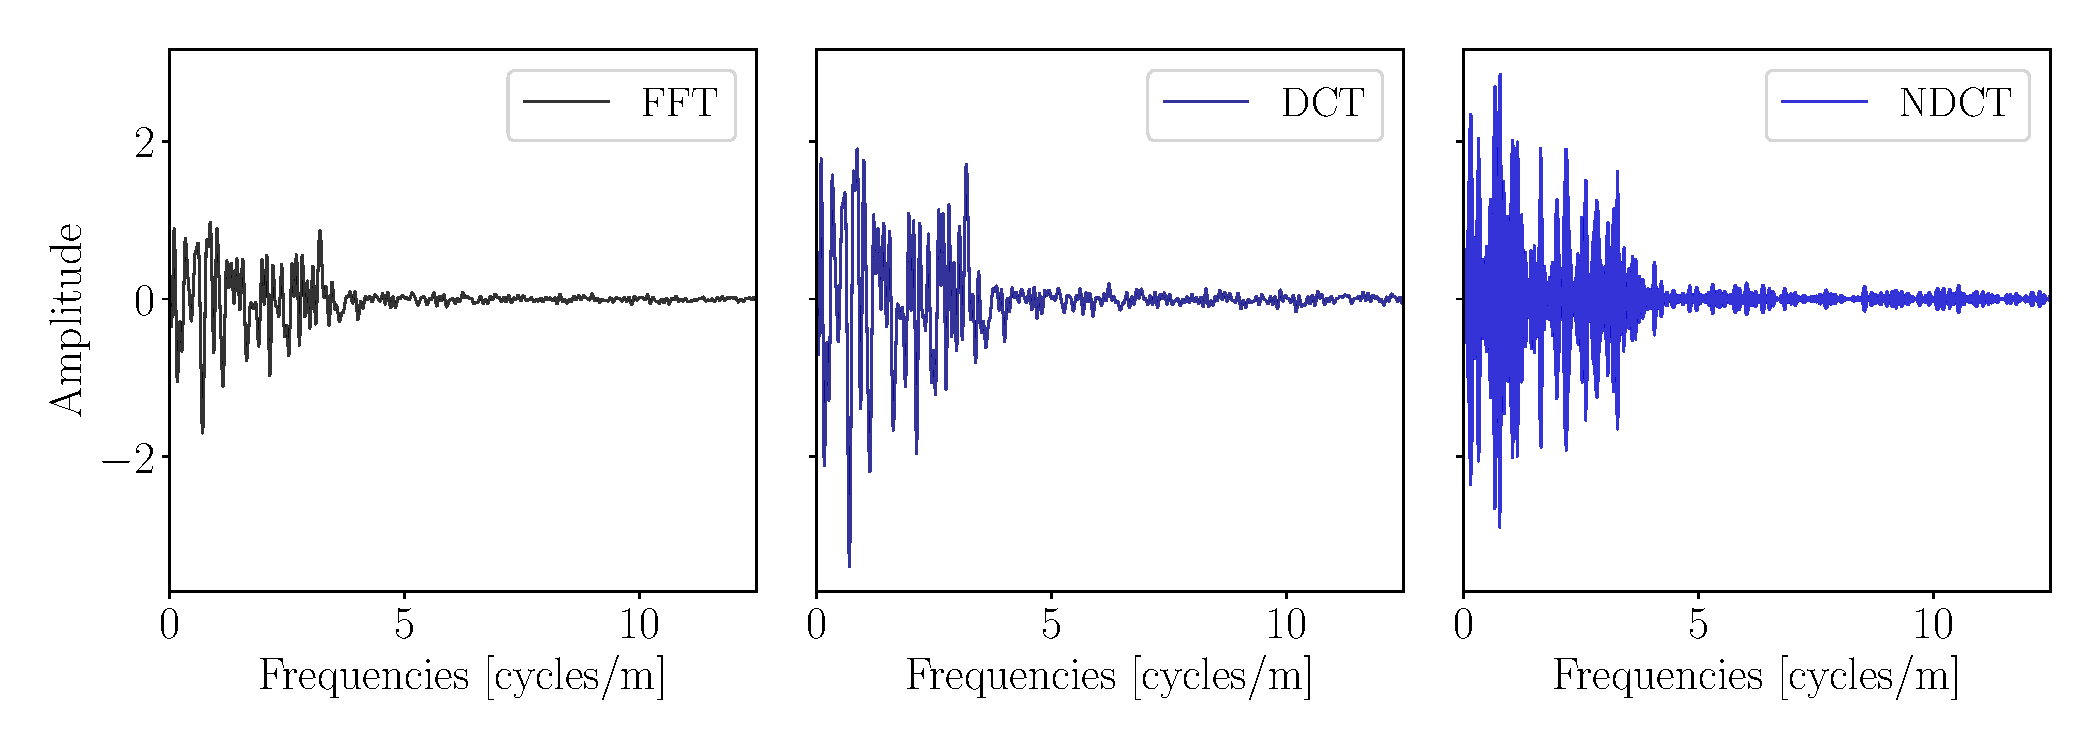
\includegraphics[width=\textwidth]{SpectralTransforms_3.pdf}
	\caption[FFT, DCT, NDCT, Site A]{\small Examples of three different spectral transforms, FFT, DCT, NDCT, performed on the depth series between Tambora and Laki eruptions from Site A.}
	\label{fig:SpectralTransforms_3}
\end{figure}

\begin{figure}[h]
	\centering
	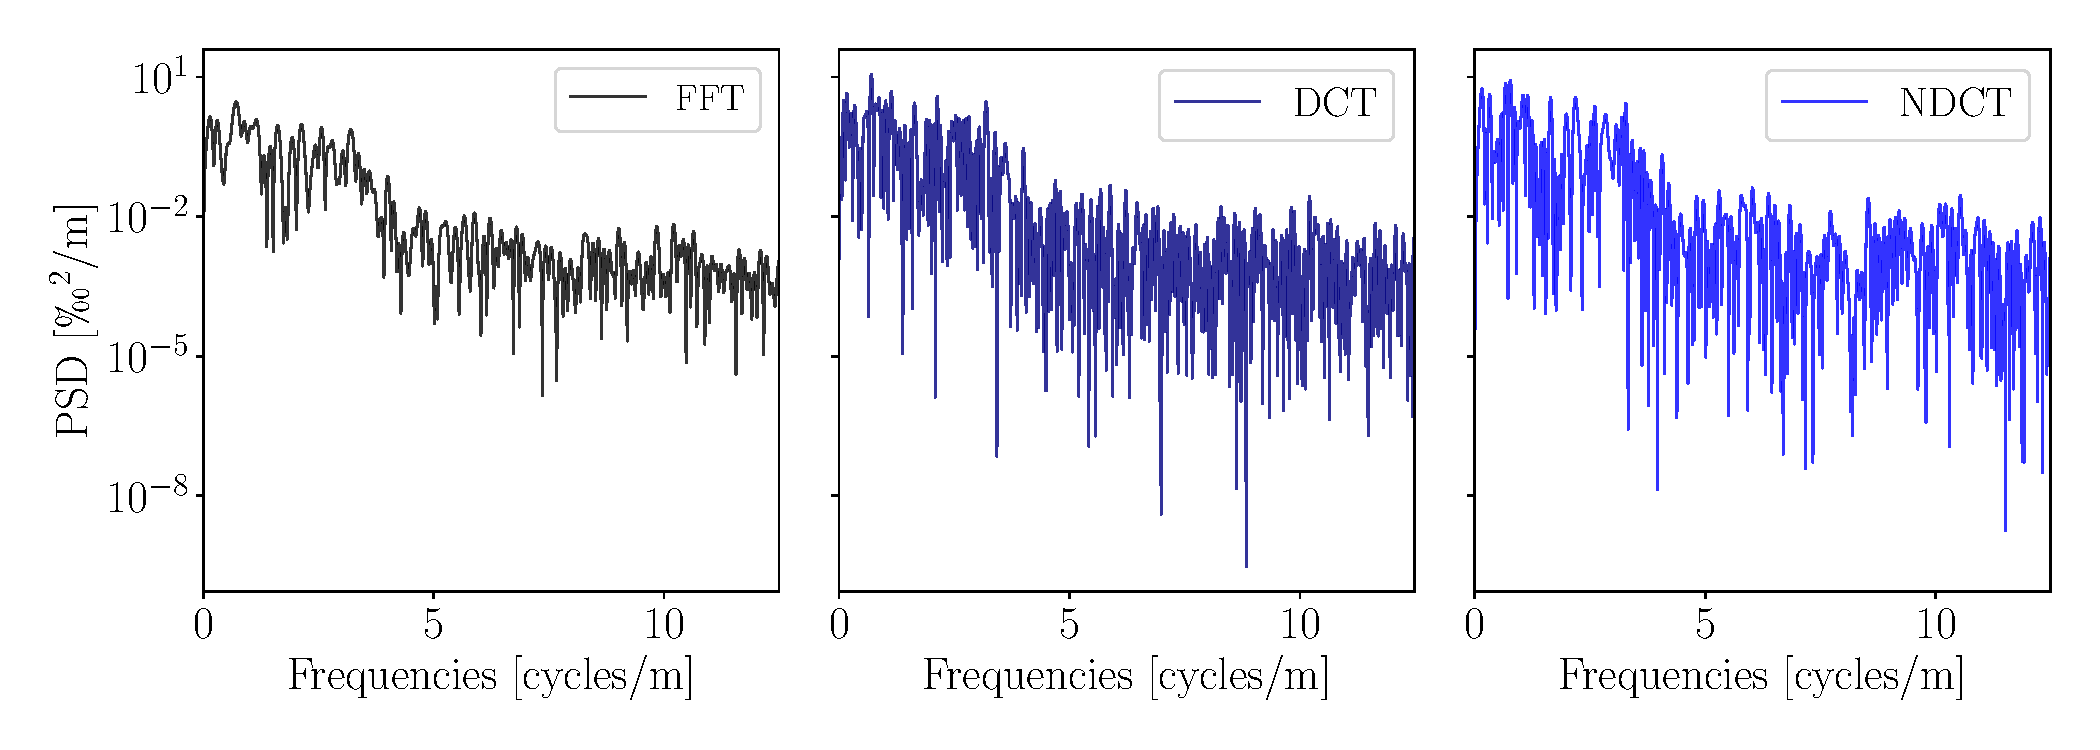
\includegraphics[width=\textwidth]{SpectralTransforms_PSD.pdf}
	\caption[FFT, DCT, NDCT PSDs, Site A]{\small Examples of power spectral densities related to the three different spectral transforms, FFT, DCT, NDCT, seen in Figure \ref{fig:SpectralTransforms_3}.}
	\label{fig:SpectralTransforms_PSD}
\end{figure}







\subsection[Signal Restoration][Signal Restoration]{Signal Restoration by Optimal Diffusion Length}
\label{Subsec:SignalAnalysis_BackDiffusion_SignalRestoration}
When considering a water isotopic depth series as the ones under examination in this thesis, it is possible to restore some of the signal lost to diffusion. This signal restoration technique will forwardly also be mentioned as 'back-diffusion', as it simulates a process that is the reverse of the diffusion process.

Along with restoring some of the signal, the spectral filtering technique used here also reveals a property of the depth series: an estimate of the diffusion length. This estimate comes from the inherent nature of the noise in the spectrum.

\subsubsection[Spectral Filtering][Spectral Filtering]{Spectral Filtering}
\label{Subsubsec:SignalAnalysis_BackDiffusion_SpectralFiltering}


When examining a real-world signal with focus on the frequency domain one will quickly run into the subject of noise. Different signals are prone to different types of noise, and must thus be treated in a fitting manner. Some spectra are prone to random low frequency noise and some to high, while others again might have a well-defined noise spectrum inherently. Understanding the nature of the noise is crucial for further signal analysis, as the signal-to-noise ratio (SNR) needs to be sufficiently high to be able to accurately separate signal and noise from each other. By understanding the noise, and modelling and estimating it, it can become possible to generate a filter which might minimize the noise and enhance the signal. This next section will go into detail with how to construct a filter fitting to the data at hand. This filtering will also be able to give an estimate of the diffusion length at a given depth section, due to the inherent nature of the signal and noise.

%
%\subsubsection{Kernel Estimation}
%\label{Subsubsec:SignalAnalysis_BackDiffusion_SignalRestoration_KernelEstimation}

Through spectral analysis it is possible to treat the noise of the signal consistently. The goal is to create spectral filters which enhances the signal while minimizing the effect of the noise, thus increasing the SNR.

Theoretically, without any diffusion, the change in isotopic concentration would be described through a step function, going from one constant concentration to another. This step function can be described by the Heaviside function:
\begin{equation}
	D(t) = \begin{cases}
		0, & t < 0 \\
		1, & t \geq
	\end{cases}
\end{equation}

In reality, a number of different mixing processes change this step function, and the measured signal will be a smooth curve, $s(t)$, which corresponds to the convolution of $S(t)$ with the mixing response function $M(\tau)$
\begin{equation}
	d(t) = \int_{- \infty}^{\infty} D(\tau) \cdot M(t - \tau)d\tau
\end{equation}

As is well known, in the spectral domain, convolution is multiplication and the mixing is described as the multiplication between the Fourier transform of $S$ and $M$:
\begin{equation}
	\tilde{d} = \tilde{D} \cdot \tilde{M}
\end{equation}


By differentiation with respect to time, the mixing filter $M$ is unaffected, and differentiation of the measured system response, the Heaviside function, $S'$ is a delta function, which Fourier transformed is unity, leading to:
\begin{equation}
	\tilde{d'} = \tilde{D'} \cdot \tilde{M} = \tilde{M}
\end{equation}

The mixing filter can thus be determined by measuring the system response to a step function, differentiating performing Fourier transform of the result $d'$.

After determination of the mixing filter $\tilde{M}$, the unmixed signal $D$ can be estimated in theory by inverse Fourier transform of


\begin{equation}
	\tilde{D} = \tilde{d}\cdot\tilde{M}^{-1}
	\label{eq:Restoration}
\end{equation}

During the mixing, cycles with short wavelengths are heavily washed out, and through the restoration in Eq. \ref{eq:Restoration}, the amplitudes corresponding to these wavelengths are heavily amplified by the filter. This method though has a drawback, which is that when the measurements contain noise, the restored signal will be dominated by high-frequency noise, greatly amplified by the mixing filter. Thus it is a problem of retaining as much (short wavelength) signal as possible while simultaneously attempting to amplify the high-frequency noise as little as possible. This optimal trade-off can be found by creating an optimum filter for the considered measured isotopic signal:
\begin{equation}
	\delta_M(z) = \delta_m (z) + \eta(z)
\end{equation} 

This optimal (Wiener) filter $\tilde{F}$, defined for each wave number $k = 2\pi \omega$, is presented as the ratio between pure signal and pure signal plus noise described in Power Spectral Densities as:
\begin{equation}
	\tilde{F}(k) =\frac{|\tilde{\delta_m}(\omega)|^2}{|\tilde{\delta_m}(\omega)|^2 + |\tilde{\eta}(\omega)|^2}
	\label{eq:WienerFilter}
\end{equation}

In this work, the power spectral densities of the signal and the noise, respectively, are determined through analysis of the power spectral density of the combined signal/noise PSD.\\
The PSD of the noise free measured signal, $|\tilde{\delta_m}(\omega)|^2$, is assumed describe as 
\begin{equation}
	|\tilde{\delta}_m(\omega)|^2 = P_0 e^{-k^2 \sigma_{\text{tot}}^2}
	\label{eq:SignalPSD}
\end{equation}
where $\sigma_{\text{tot}}^2$ describes the total estimated diffusion length of the mixing.\\
The noise is assumed to be red noise, described by an autoregressive process of first order, AR1:
\begin{equation}
	|\tilde{\eta}(\omega)|^2 = \frac{\sigma_{\eta}^2 \Delta z}{|1 + a_1 \exp(-2\pi i \omega \Delta z)|^2}
	\label{eq:NoisePSD}
\end{equation}
where $\sigma_{\eta}^2$ is the variance of the red noise, $a_1$ is the AR1 coefficient and $\Delta z$ is the resolution of the time/depth data.
It is then possible to estimate the parameters $P_0$, $\sigma_{\text{tot}}^2$, $\sigma_{\eta}^2$ and $a_1$ by curve fitting, separately, the two expressions in Eq. \ref{eq:SignalPSD} and \ref{eq:NoisePSD} to the data. The estimated parameters are varied to find the optimal guess to use for the filter.

\begin{figure}
	\centering
	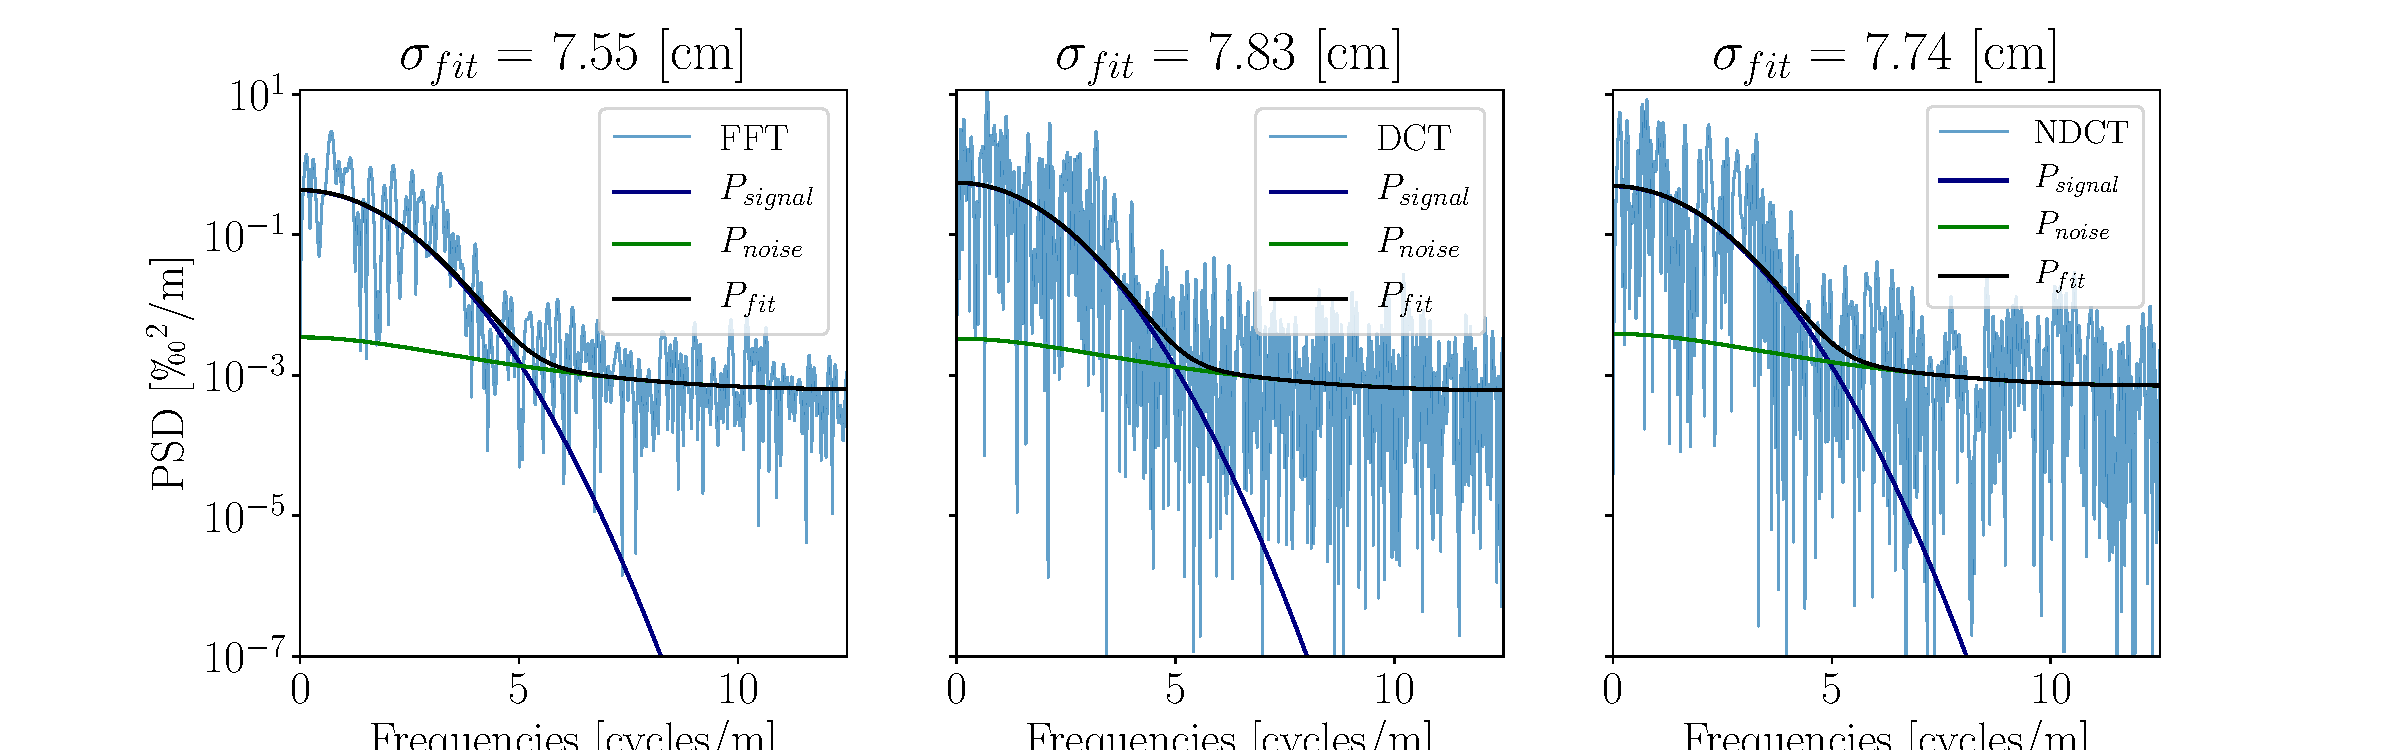
\includegraphics[width=\textwidth]{SpectralTransforms_PSDwFits.pdf}
	\caption[FFT, DCT, NDCT PSDs with Fit, Site A]{\small Noise, signal and total fit to PSD, illustrating the construction of the Wiener Filter, see Sec. \ref{Sec:SignalAnalysis_Restoration}.}
	\label{fig:SpectralTransforms_PSDwFits}
\end{figure}

An example of the constructed Wiener filter can be seen in Figure \ref{fig:SiteA_WienerFilters} on both a linear and a double logarithmic scale.


\begin{marginfigure}
	\centering
	\begin{subfigure}{\marginparwidth}
		\centering
		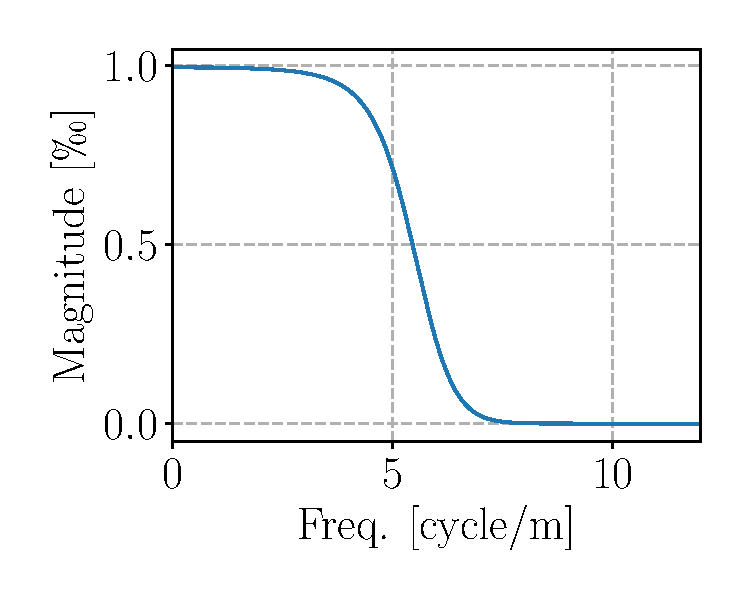
\includegraphics[width=\textwidth]{SiteA_WienerFilter.pdf}
		\caption{\footnotesize}
		\label{fig:SiteA_WienerFilter}
	\end{subfigure}\\[1ex]
	
	\begin{subfigure}{\marginparwidth}
		\centering
		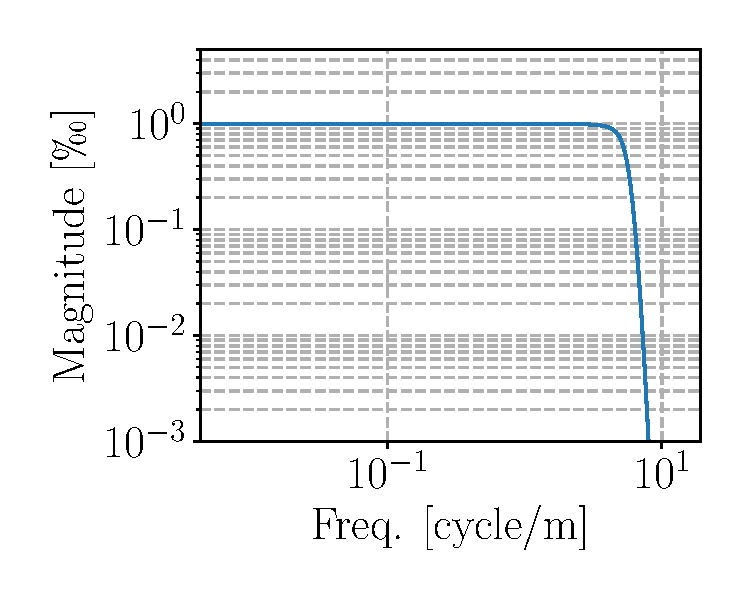
\includegraphics[width=\textwidth]{SiteA_WienerFilter_loglog.pdf}
		\caption{\footnotesize}
		\label{fig:SiteA_WienerFilter_loglog}
	\end{subfigure}
	\caption[Wiener filter]{\footnotesize\textbf{(a)} Wiener filter on linear scale. \textbf{(b)} Wiener filter on double logarithmic scale.}
	\label{fig:SiteA_WienerFilters}
\end{marginfigure}

\subsubsection[Final Restoration][Final Restoration]{Final Restoration}
\label{Subsubsec:SignalAnalysis_BackDiffusion_FinalRestoration}

After finding the best fit (noise and signal) to the spectral data, it is possible to construct an optimal restoration filter, $\tilde{R}$, which contains two separate filters. The one is the Wiener filter, $\tilde{F}$, which is described in the above section and the other is a Gaussian filter constructed to amplify certain frequencies [REFERENCE]. This filter, the transfer function of the system, is constructed to specifically amplify the frequencies heavily attenuated by the diffusion process and is described as
\begin{equation}
	\mathcal{G} = \frac{1}{\sigma\sqrt{2\pi}} e^{\frac{-z^2}{2\sigma^2}},
	\label{Eq:TransferFct_z}
\end{equation}
in the time(depth) domain and, since the Fourier transform of a Gauss is still a Gauss, in the frequency domain it is described as:
\begin{equation}
	\tilde{\mathcal{G}} = \mathcal{F}[\mathcal{G(z)}] = e^{\frac{-(2\pi\, f)^2\sigma^2}{2}}.
	\label{Eq:TransferFct_frq}
\end{equation}

Finally, the constructed frequency restoration filter, in the frequency domain, is a product of the Wiener filter, from Eq. \ref{eq:WienerFilter}, and the transfer function, from Eq. \ref{Eq:TransferFct_frq}:

\begin{equation}
	\tilde{R} =  \tilde{F} \cdot \tilde{\mathcal{G}}^{-1}
\end{equation}
which results in a rewrite of equation \ref{eq:Restoration} to:
\begin{equation}
	\tilde{D} = \tilde{d}\cdot\tilde{F}\cdot\tilde{\mathcal{G}}^{-1}
\end{equation}

An example of the final frequency restoration filter, as it changes with diffusion length estimate inputted in the transfer function, $\tilde{\mathcal{G}}$, can be seen in Figure \ref{fig:SiteA_filtersEx}.

\begin{figure}[h]
	\centering
	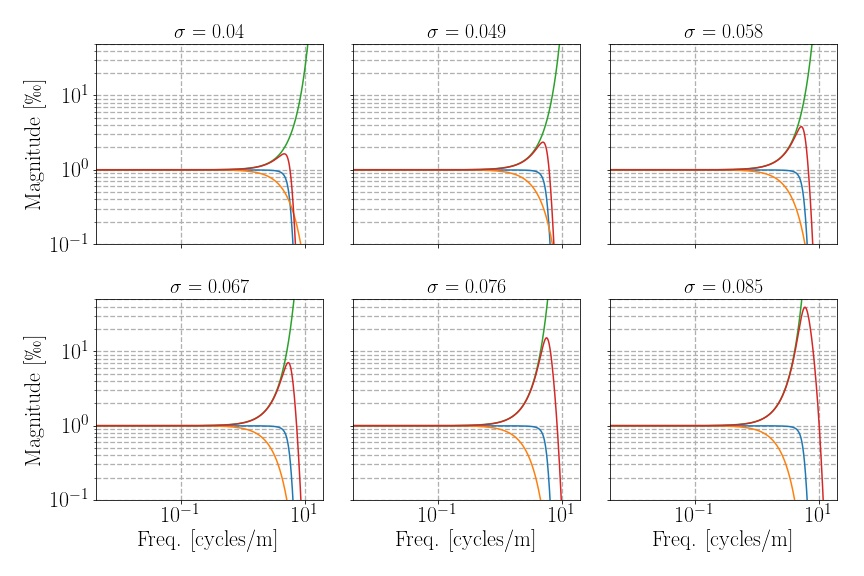
\includegraphics[width=\textwidth]{SiteA_filtersEx.jpg}
	\caption[Frequency filters example, Site A]{\small Frequency filter examples ranging from diffusion length 0.04 m to 0.085 m.}
	\label{fig:SiteA_filtersEx}
\end{figure}


\subsection[ALT from Spectral Analysis]{Annual Layer Thickness Estimates}
\label{Subsubsec:SignalAnalysis_SpectralAnalysis_ALT}

The transfer function of the diffusion process, Eq. \ref{Eq:TransferFct_frq}, can be rewritten as a function of the wavelength of the isotopic signal, $\lambda$:
\begin{equation}
	\tilde{\mathcal{G}} = e^{\frac{-2\pi^2\sigma^2}{\lambda^2}}
	\label{Eq:TransferFct_lambda}
\end{equation}

The wavelength of the signal corresponds roughly to the annual layer thickness, $\lambda_A$, in the signal. Regarding the isotopic signal as a wave, it is clear from both theoretical knowledge of the processes and visual inspection of the data, that the diffusion and densification have an effect on the magnitude and the wavelength/frequency respectively. The diffusion attenuates some of the waves magnitude, and the densification shortens the wavelength of the signal. Since both magnitude and wavelength are aspects of a wave, the general effects of the densification and diffusion processes can be examined by spectral analyzing the entire core. This is done by dividing the signal into a number of sections of an (almost) fixed length, $l_{sec}$ and shifting this section down through the core with a shift of length $l_{shift}$. The length is not exactly fixed, as the sample sizes vary through the core, which results in small variations in section and shift lengths.

From the spectral analysis, an estimate on the annual layer thickness can be given, corresponding to the most prominent frequency peak in the spectrum. Sometimes, though, the most prominent peak might be a resonance frequency at some value below that of the frequency related to the $\lambda_A$. This has been dealt with in this thesis by simply assuming that the frequency in section $l_{sec}^i$ must be larger than the frequency in $l_{sec}^{i-1}$, and the analysis is then carried out be sequentially going through the depth segments. Since different spectral transforms have already been introduced, it was obvious to compute the spectral analysis and most prominent frequency through more than one spectral transform. Thus DCT, NDCT, FFT and MEM has been used, and the found frequencies have then been used to estimate and average wavelength, and thereby $\lambda_A$, in the given section, see Figure \ref{Fig:SiteB_0-5m_ALTestimate_example} showing a spectral analysis with 4 different transforms of the first 5 meters of the core drilled at Site B.

\begin{marginfigure}
	\centering
	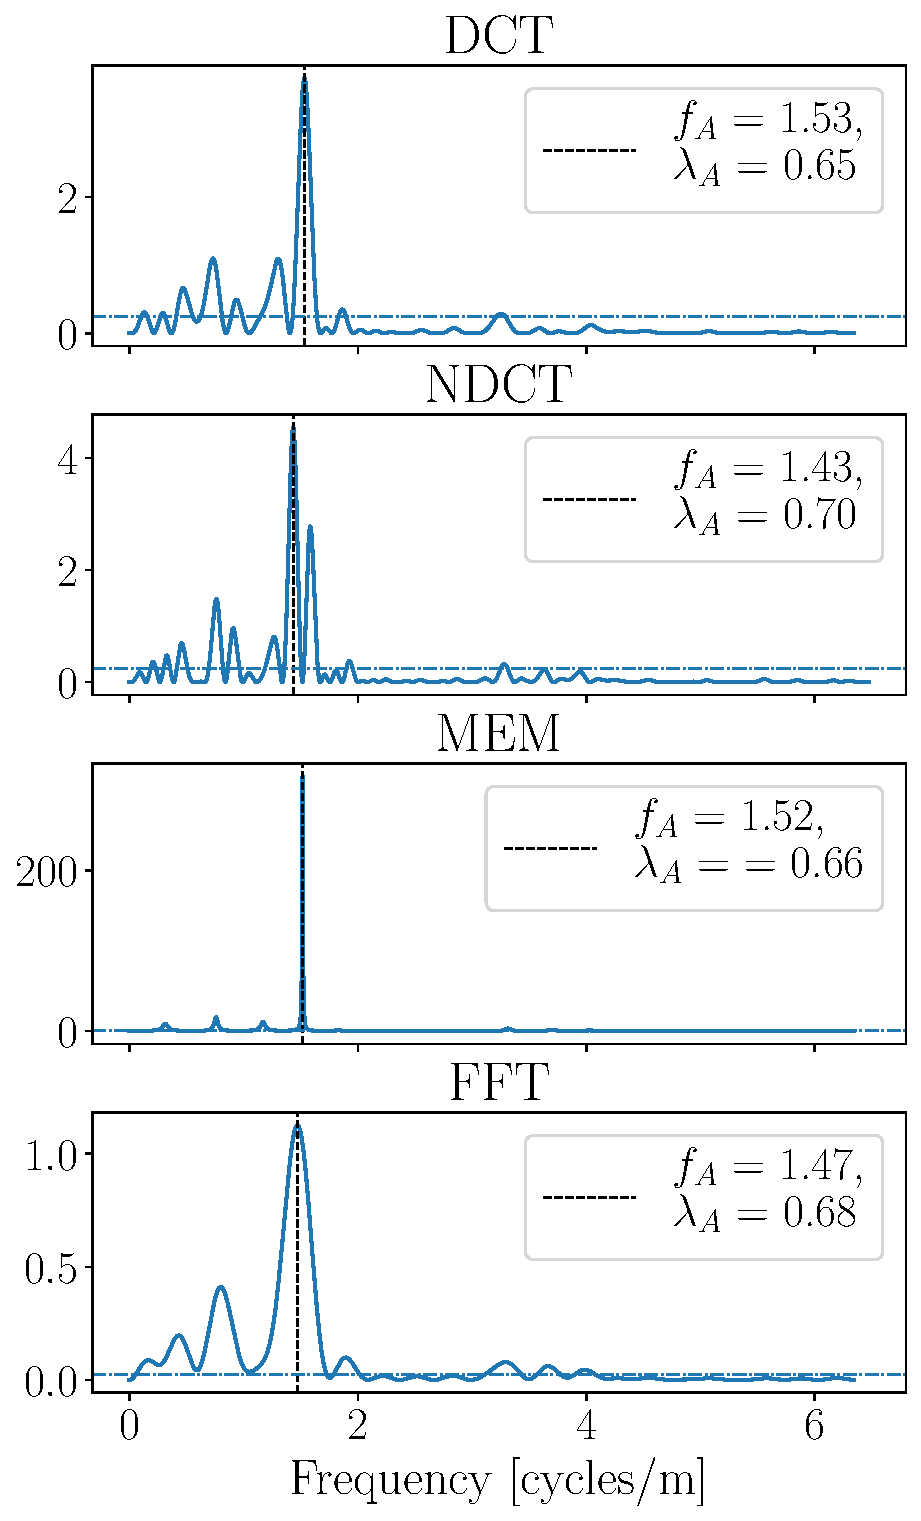
\includegraphics[width=\marginparwidth]{SiteBALTestimate_example.pdf}
	\caption[$\lambda$ estimation example, Site B, in frequency domain.]{\footnotesize Example of annual layer thickness estimation for section of 5 meters at depth [0;5] m, Site B.}
	\label{Fig:SiteB_0-5m_ALTestimate_example}
\end{marginfigure}
%
%\begin{figure}[h]
%	\centering
%	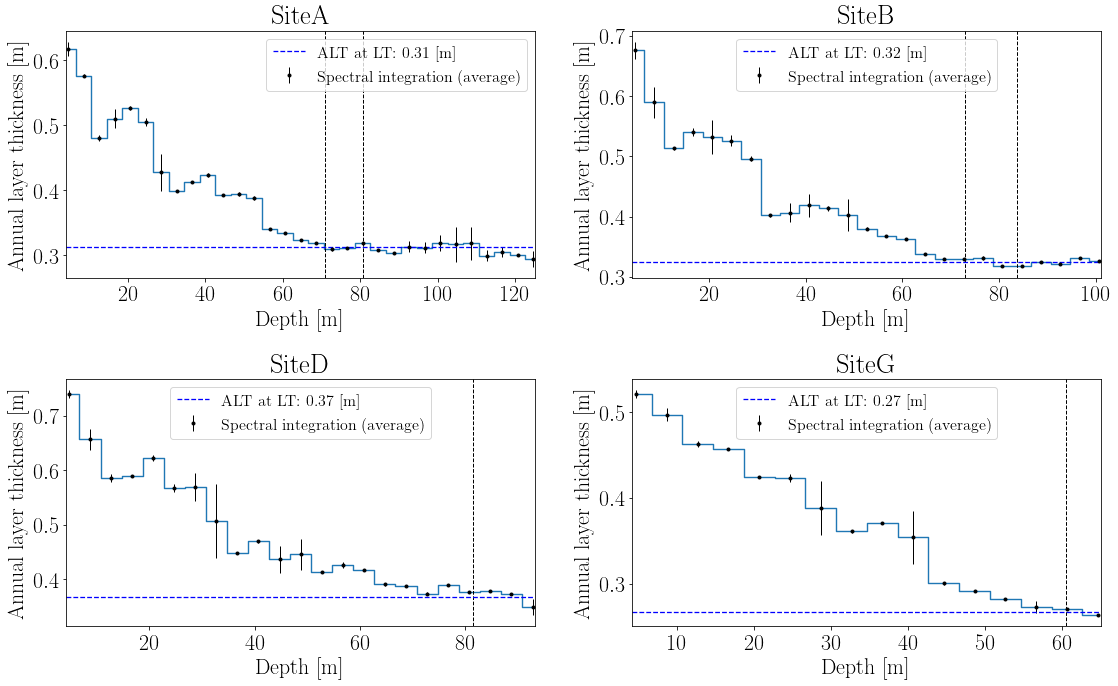
\includegraphics[width=0.95\textwidth]{AllCores_ALT_l5_s4.png}
%	\caption[$\lambda$ profiles for sites A, B, D and G.]{\small Annual layer thickness as estimated through spectral analysis, with a section length of 5 m and a section shift of 4 m, Sites A, B, D and G.}
%	\label{Fig:AllCores_ALT_l5_s4}
%\end{figure}

Figure \ref{Fig:AllCores_ALT_l5_s4} shows the $\lambda_A$ estimates of the entire cores drilled at site A, B, D and G. The section length is 5 m and the shift is 4 m, to avoid missing any frequencies in the transitions between sections. Along with the estimated $\lambda_A$s, an estimate of the average $\bar{\lambda}_A$ value at the depth corresponding to between Laki and Tambora events has also been shown. 


\begin{figure}[h]
	\centering
	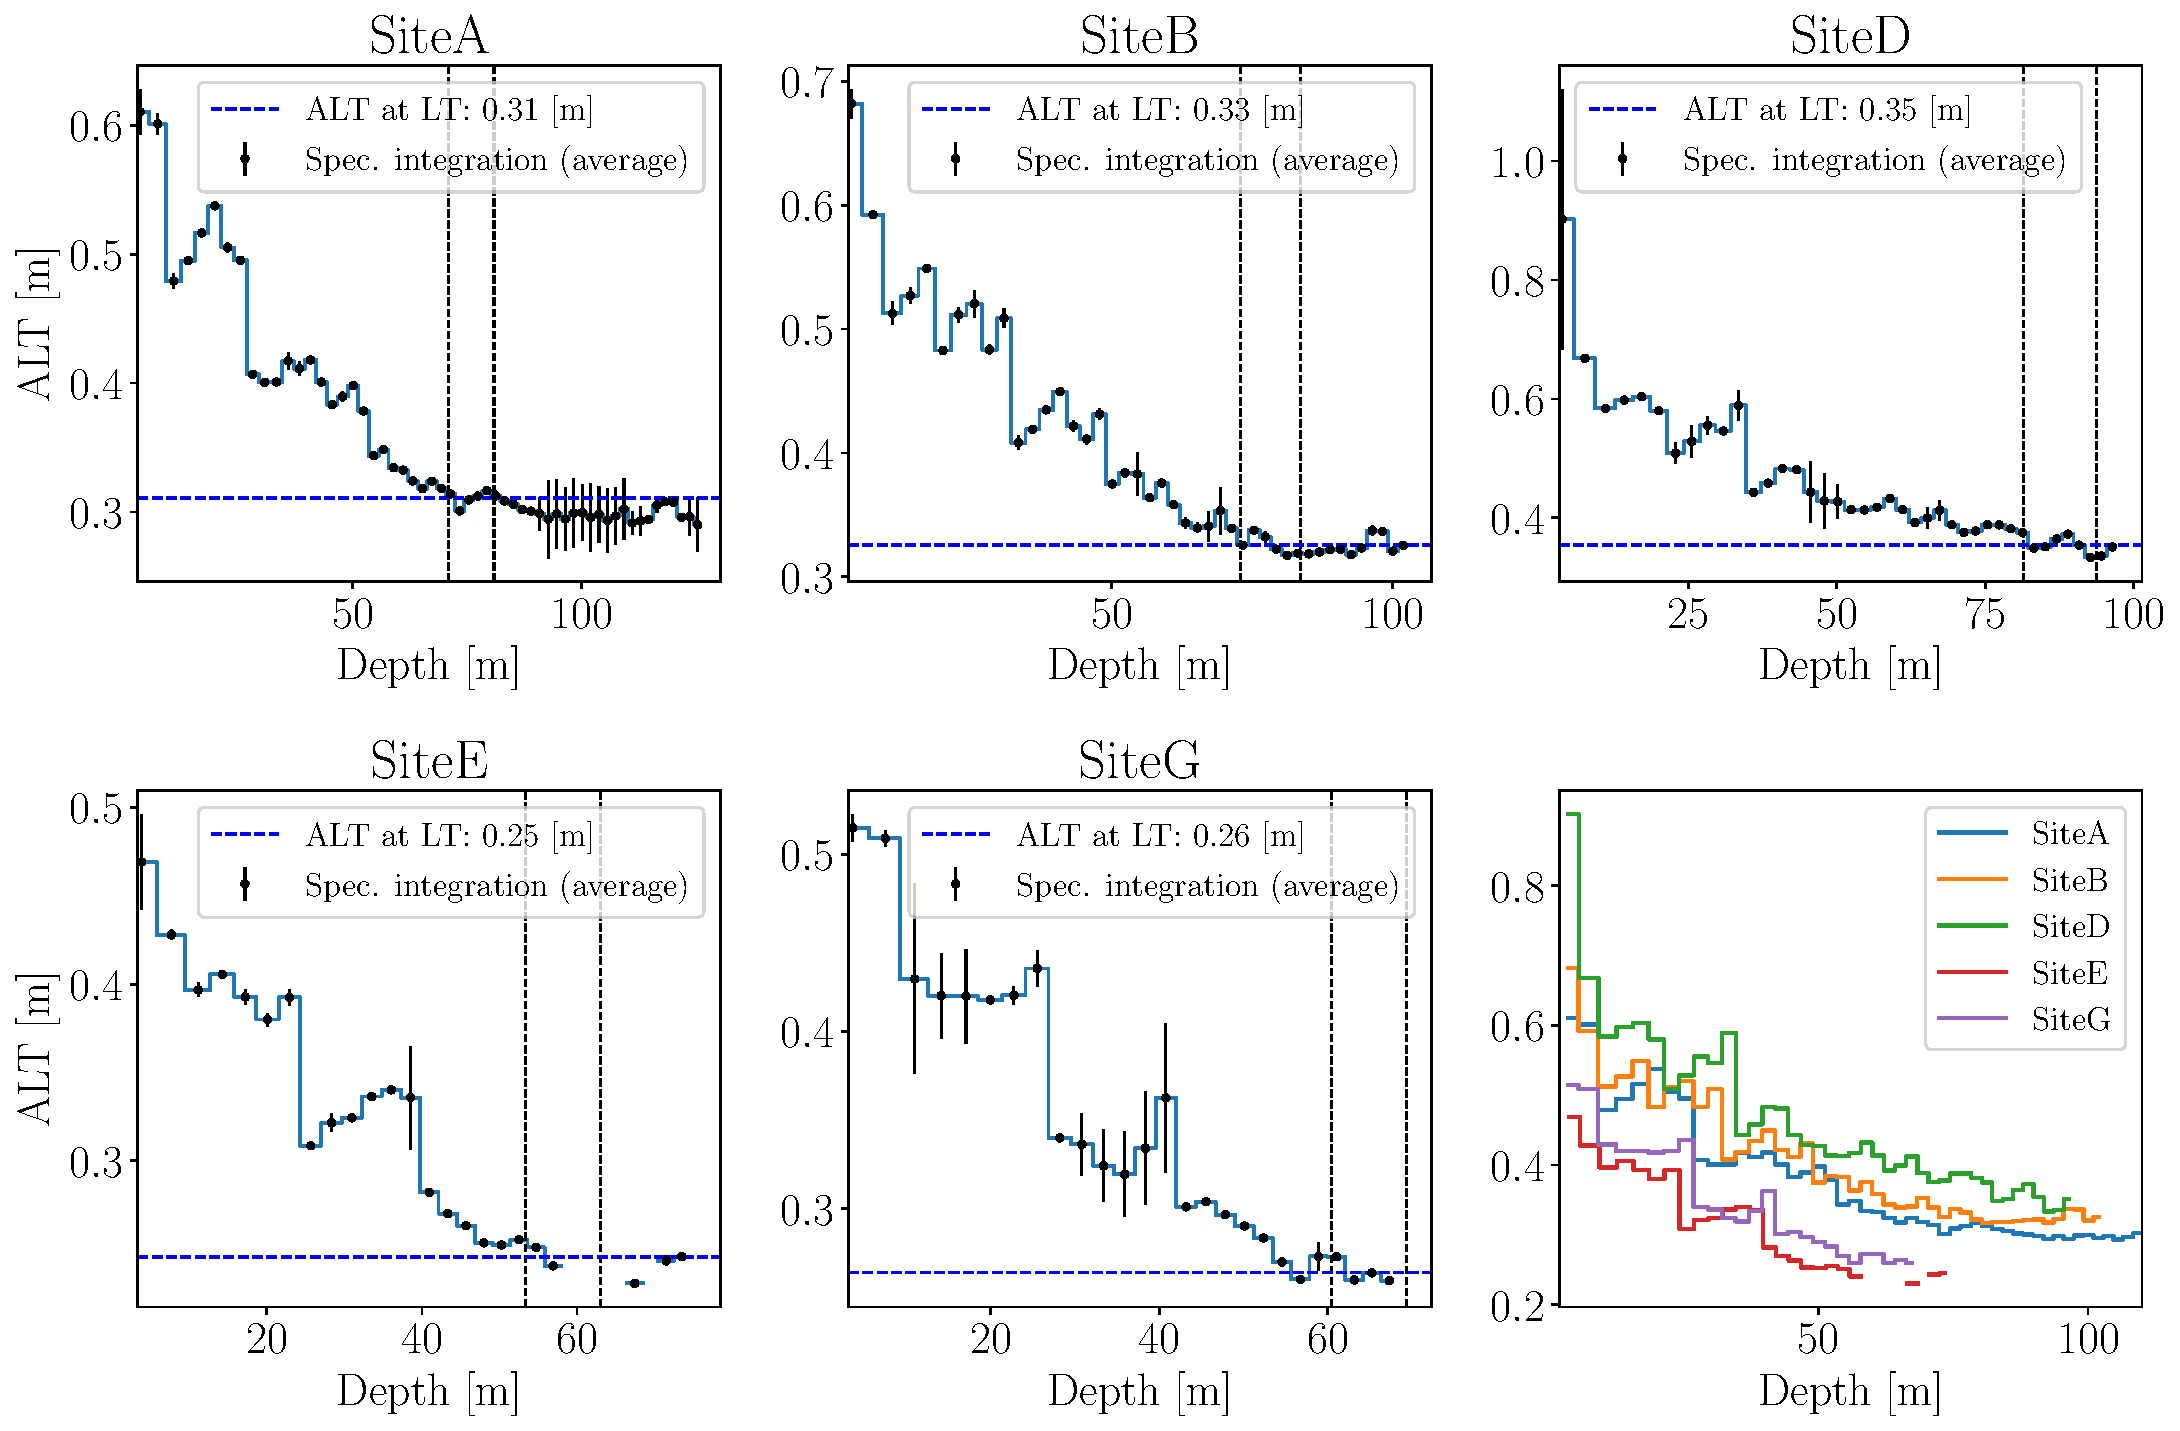
\includegraphics[width=0.95\textwidth]{AllCores_ALTs.pdf}
	\caption[$\lambda$ for Full Cores]{\small Annual layer thickness estimates, $\lambda$, calculated through spectral integration of 5 m sections of the entire core lengths. The average is based on using both FFT, DCT and NDCT spectral estimations. Blank spaces, akin to the sections below 60 m depth at Site E shows problematic areas, where the spectral estimation have had trouble with determining $\lambda$. The black vertical lines show the depth sections between Laki and Tambora events.}
	\label{fig:AllCores_ALT_l5_s4}
\end{figure}

Estimating $\lambda_A$ is dependent on both the length of the section on which the spectral analysis is performed and on the length of the shift between spectral estimates. The final $\lambda_{\text{LT}}$ used as a constraint on peak distance in the final algorithm is determined as an average of the estimated $\lambda_A$ falling inside the Laki to Tambora depth interval.

\subsubsection[Change in $l_{sec}$]{Change in section length}
\label{Subsubsec:SignalAnalysis_SpectralAnalysis_ALT_lsec}

When performing spectral analysis on a time series, the length of the section under examination is crucial for the outcome of the analysis. If the section is too short to contain the information hidden in the signal, then it will be difficult to detect patterns and frequencies of interest. If the section is too long though, too many features that are just noise might be enhanced. Furthermore, for a nonlinear signal as the isotopic depth series are, the linearity does not hold for very long sections, as the cycles are compressed and diffused. Thus it is of interest to examine the effect of the section length on the annual layer thickness estimates. The $\lambda_A$ estimates where performed for sections lengths of ?? to ?? m. Above this upper limit, there where too much noise in the spectrum to determine a $\lambda_A$.

In Figure \ref{Fig:AllCores_ALT_at_DiffLsecs} different $\lambda_A$ depth profiles can be seen, given five different section lengths. All estimates are made with a shift of 1 m. Considering the shortest section length of $l_{sec}=1.00$ m, it is clear that the estimation method picks up some noise resulting in a highly varying $\lambda_A$ estimate throughout the cores. but, generally, the other four section lengths seem to pick up the same annual cycles, except for at Site E and G, where the two largest section lengths of 15.55 m and 20.39 m give some very long annual layer thicknesses at some depths.

Considering Figure \ref{Fig:AllCores_ALTatLT_vs_lSec} the $\lambda_A$ estimates  of the Laki to Tambora depth sectionsshow low stability at short section lengths and increasing accuracy and precision as the section length increases, until at some point, especially clear in Site E, but also visible in Site G and Site A, the accuracy start to drop as the variance of the $\lambda_{\text{LT}}$ estimate increases.
\begin{figure}[h]
	\centering
	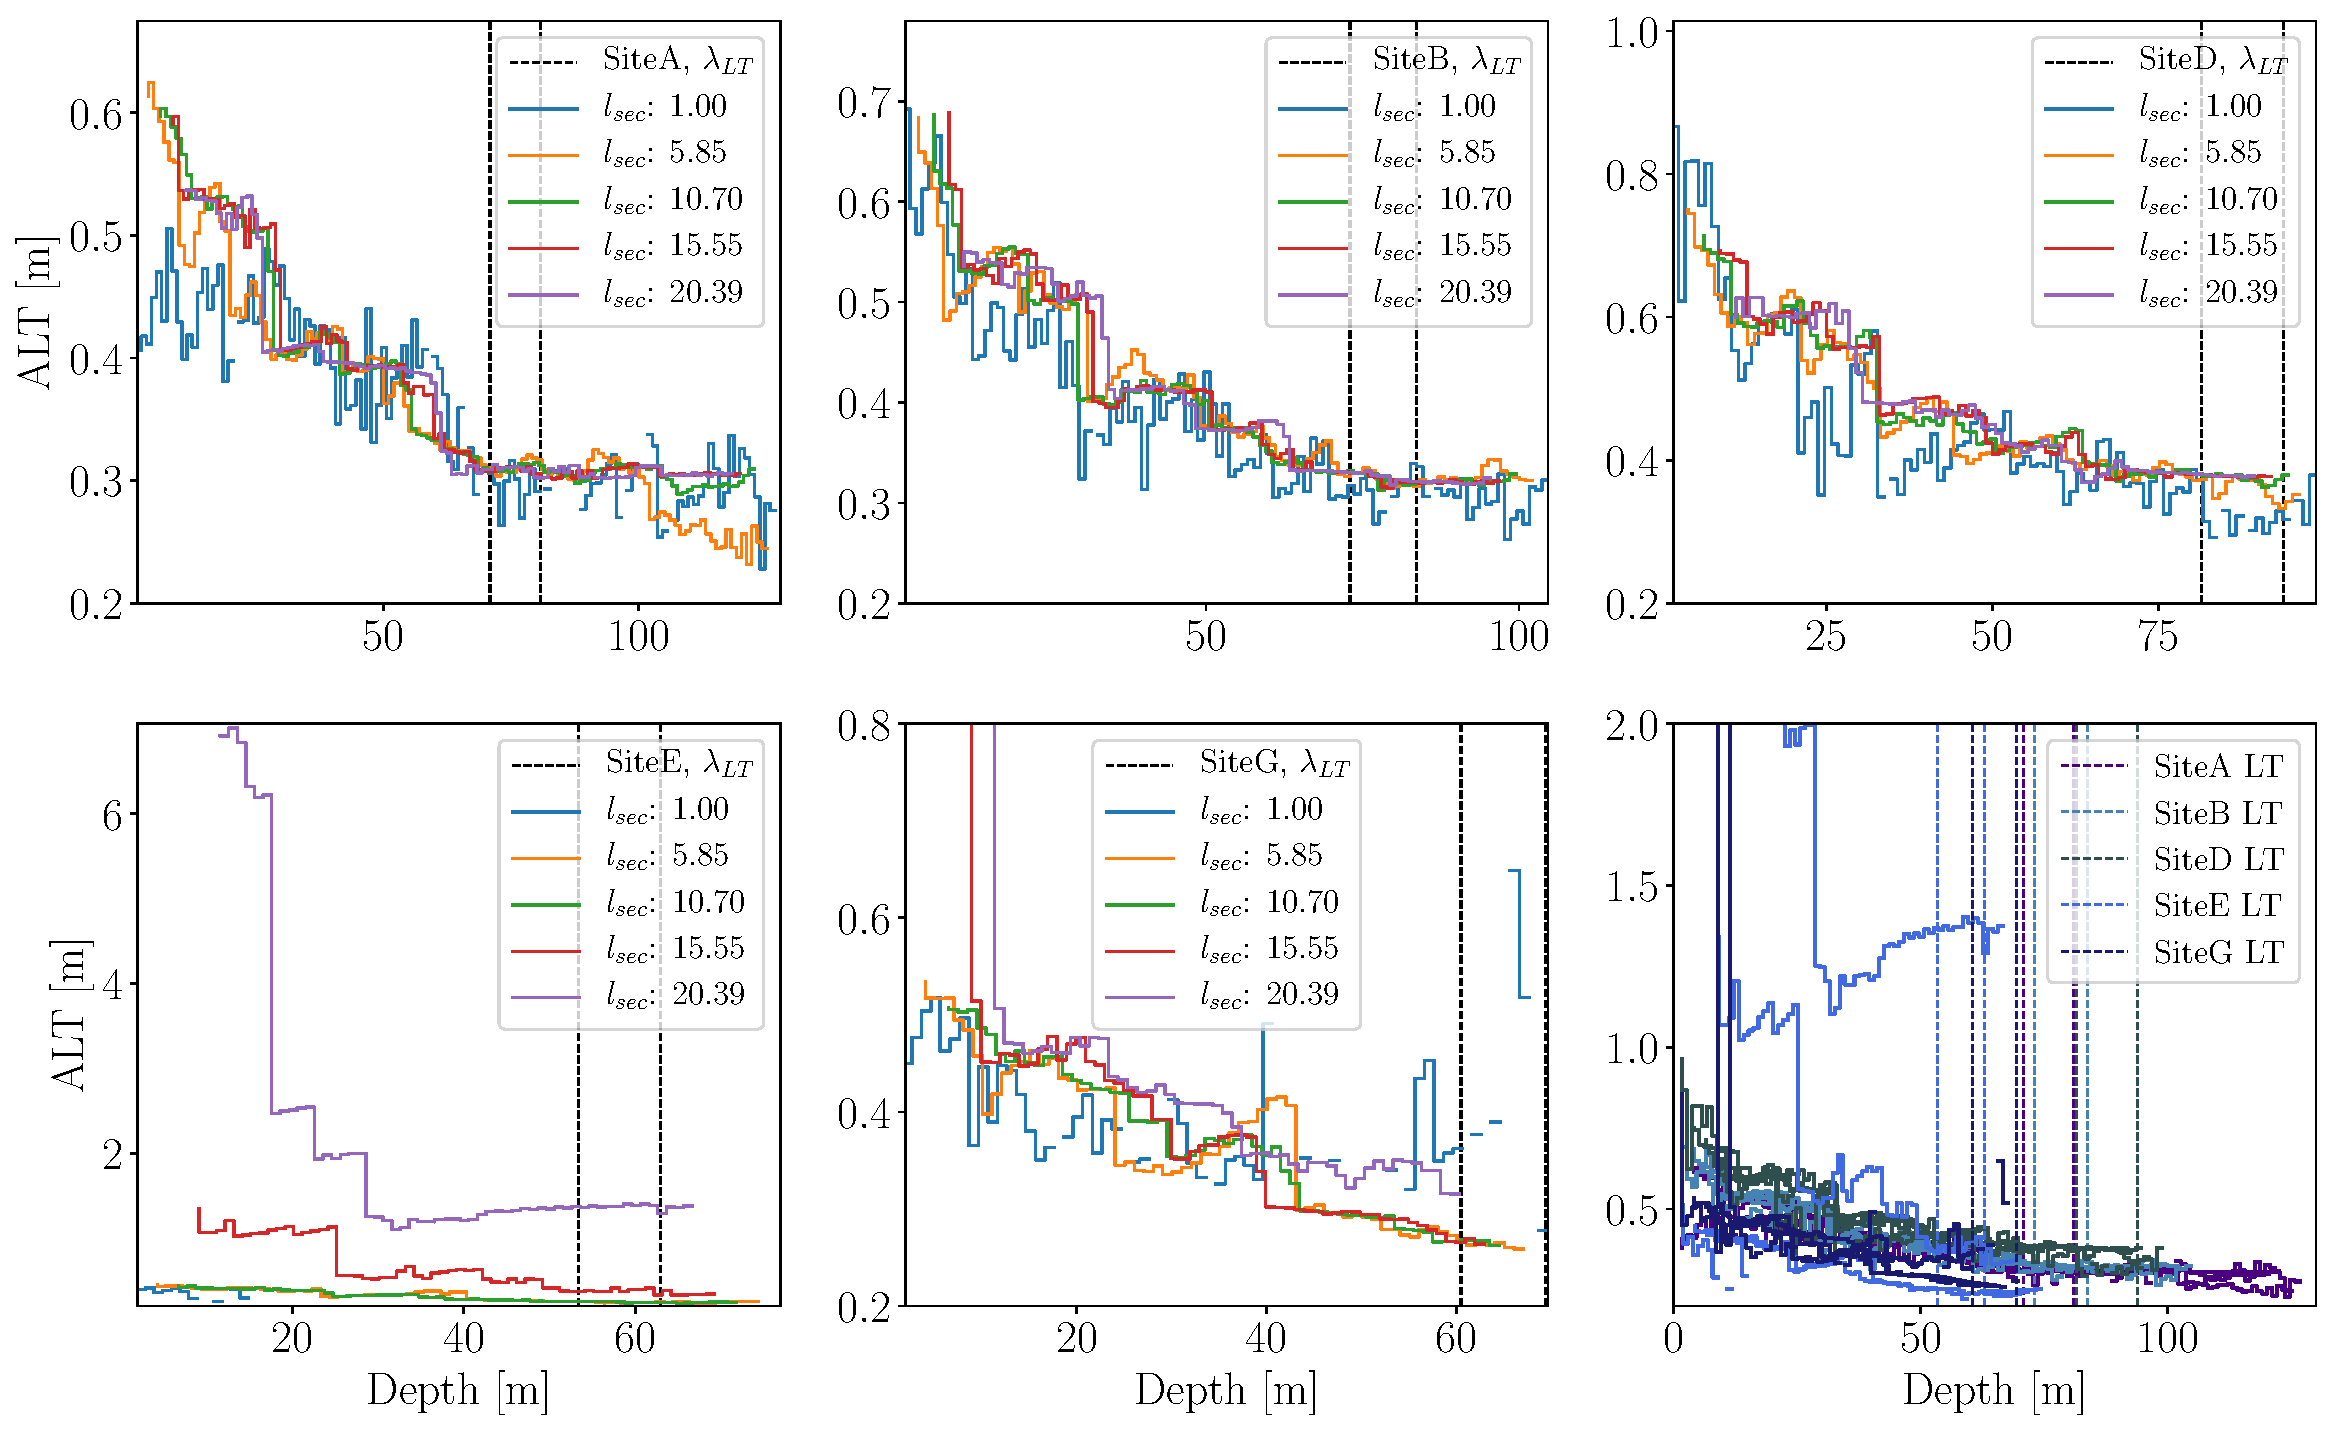
\includegraphics[width=\textwidth]{AllCores_ALT_at_DiffLsecs.pdf}
	\caption[$\lambda$ Depth Profiles, Different $l_{\text{sec}}$]{\small Examples of the $\lambda$ depth profile given different section lengths. All profiles are computed with a shift of 1 m.}
	\label{fig:AllCores_ALT_at_DiffLsecs}
\end{figure}

\begin{figure}[h]
	\centering
	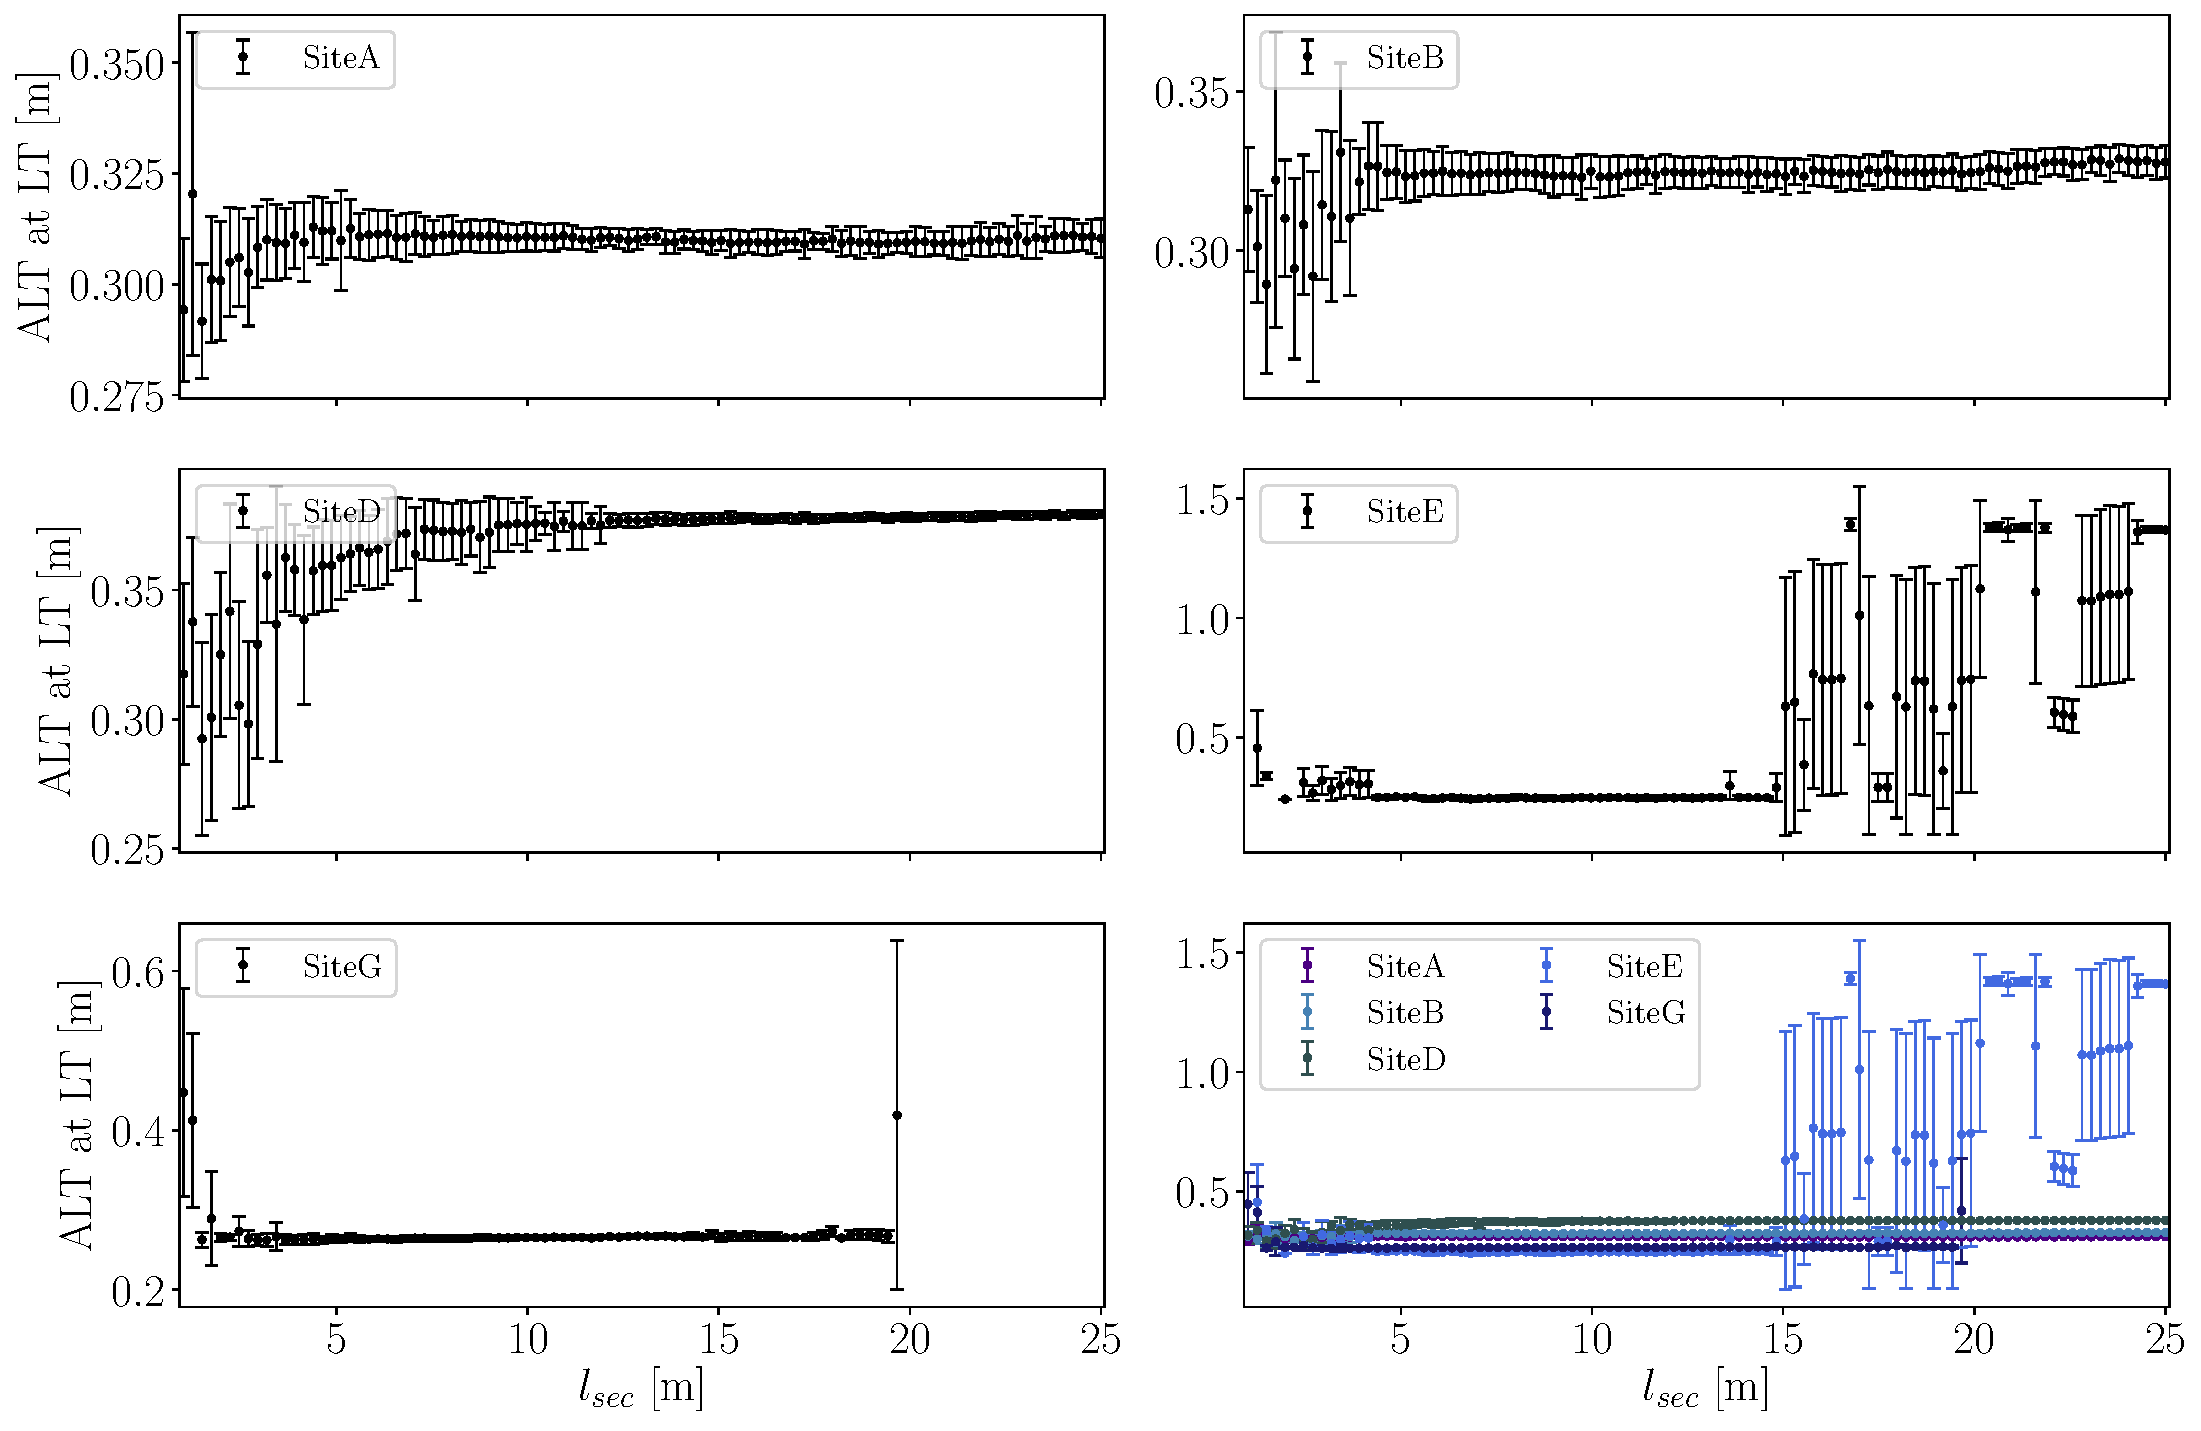
\includegraphics[width=\textwidth]{AllCores_ALTatLT_vs_lSec.pdf}
	\caption[$\lambda_{\text{LT}}$ vs. Section Length]{\small The annual layer thickness estimates in the section between Laki and Tambora as computed with different section lengths, $l_{\text{sec}}$, used in the spectral analysis. The section is shifted 1 m and then computed again. The $\lambda_{\text{LT}}$ is then calculated as a mean of th $\lambda$ estimates falling into the Laki to Tambora depth section.}
	\label{fig:AllCores_ALTatLT_vs_lSec}
\end{figure}

Based on the stability analysis of the section lengths, the general section length to estimate $\lambda_A$ in this work was set to $\lambda_A=7$ m, but with possibility to vary.


\subsubsection[Change in $l_{shift}$]{Change in shift length}
\label{Subsubsec:SignalAnalysis_SpectralAnalysis_ALT_lshift}
The change in shift length is assumed to be more an issue of how detailed the $\lambda_A$ depth profile needs to be versus how computationally fast it is needed to be. If the shift is small, there will be a need to perform the spectral analysis many times before the entire depth is covered, but many small varying features may become visible throughout the core. All shift lengths are examined with a section length of $\l_{sec}=7$ m.

For this project though, a rough estimate of the $\lambda_{\text{LT}}$ at a given depth is needed, and the accuracy and details is not as important. Looking at Figure \ref{Fig:AllCores_ALT_at_DiffShifts} it is obvious that for most cores there is a clear exponential attenuation effect on the layer thickness. This effect is visible for all different shift lengths, which might point to that, for this work at least, a very small shift is not necessary.

Interestingly, though, is that especially for Site E and Site G, there are some depths where the $\lambda_A$ estimates seem to be increasing instead of decreasing. Luckily for this work, these depth are not of interest, and the specific depth between the Laki and Tambora events seem to be stable at almost any shift length. Only site E presents some troubles where $\lambda_A$ has presented itself difficult to estimate exactly at the Laki to Tambora depth. For this specific core it could therefore be necessary to decrease the shift length to be able to get more estimates in the Laki to Tambora area.
\begin{figure}[h]
	\centering
	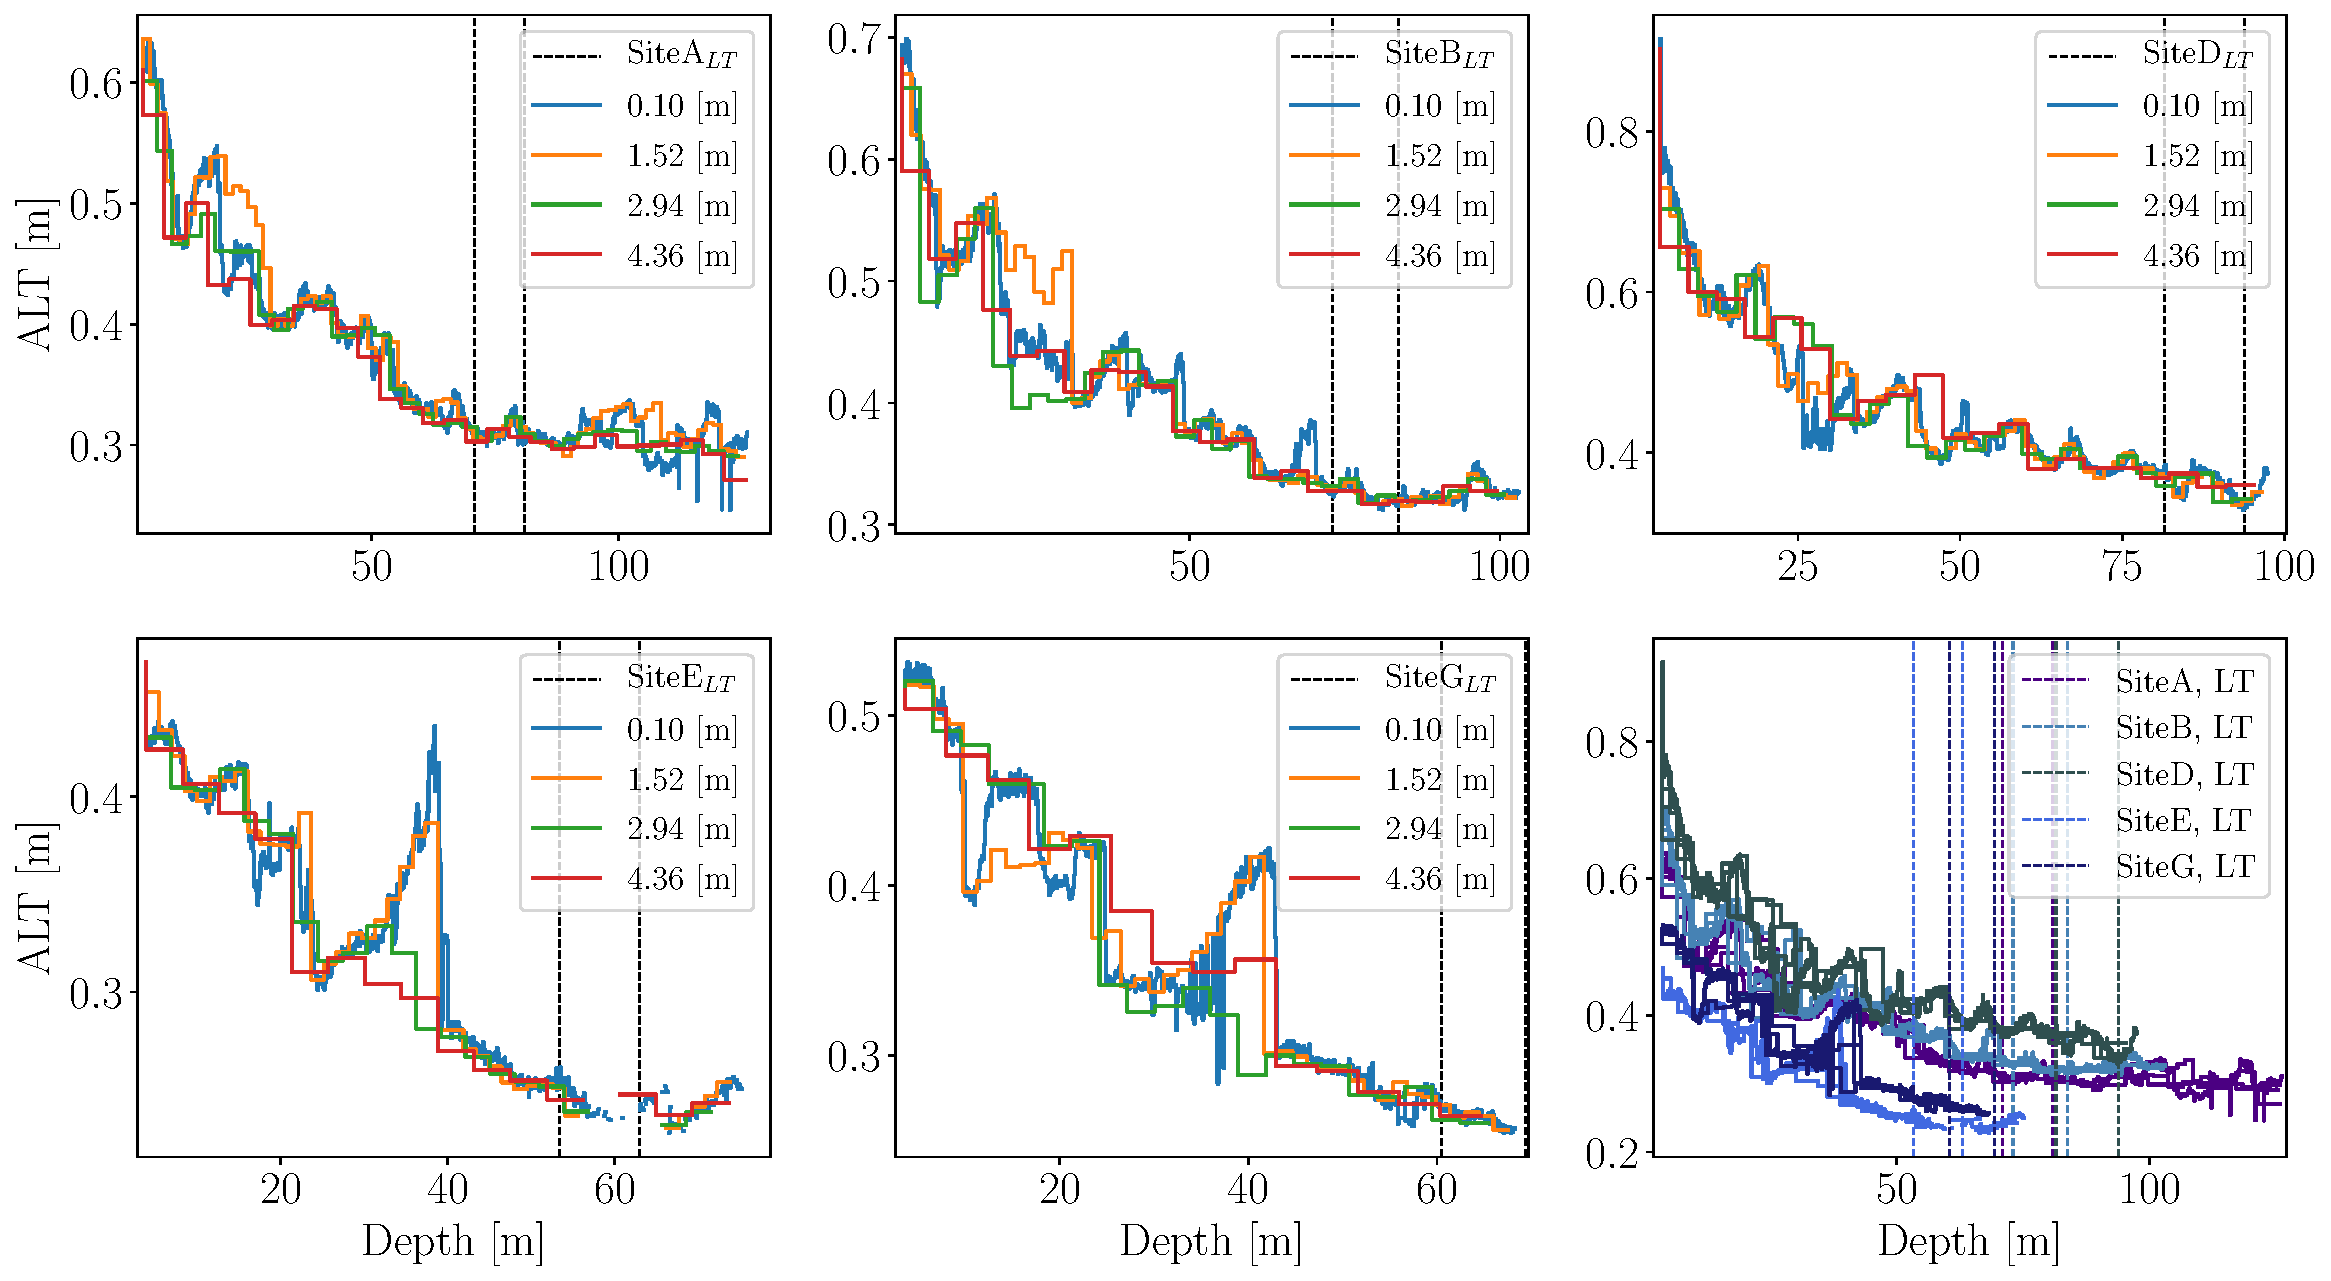
\includegraphics[width=\textwidth]{AllCores_ALT_at_DiffShifts.pdf}
	\caption[$\lambda$ Depth Profiles, Different $s_{\text{sec}}$]{\small Examples of $\lambda$ depth profiles given different shift lengths. All profiles are computed with a section length for spectral analysis of $l_{\text{sec}}=5$ m.}
	\label{fig:AllCores_ALT_at_DiffShifts}
\end{figure}

In Figure \ref{Fig:AllCores_ALTvsShift} the $\lambda_{\text{LT}}$ versus shift length can be seen, with shifts from 0.05 m to 5 m.

\begin{figure}[h]
	\centering
	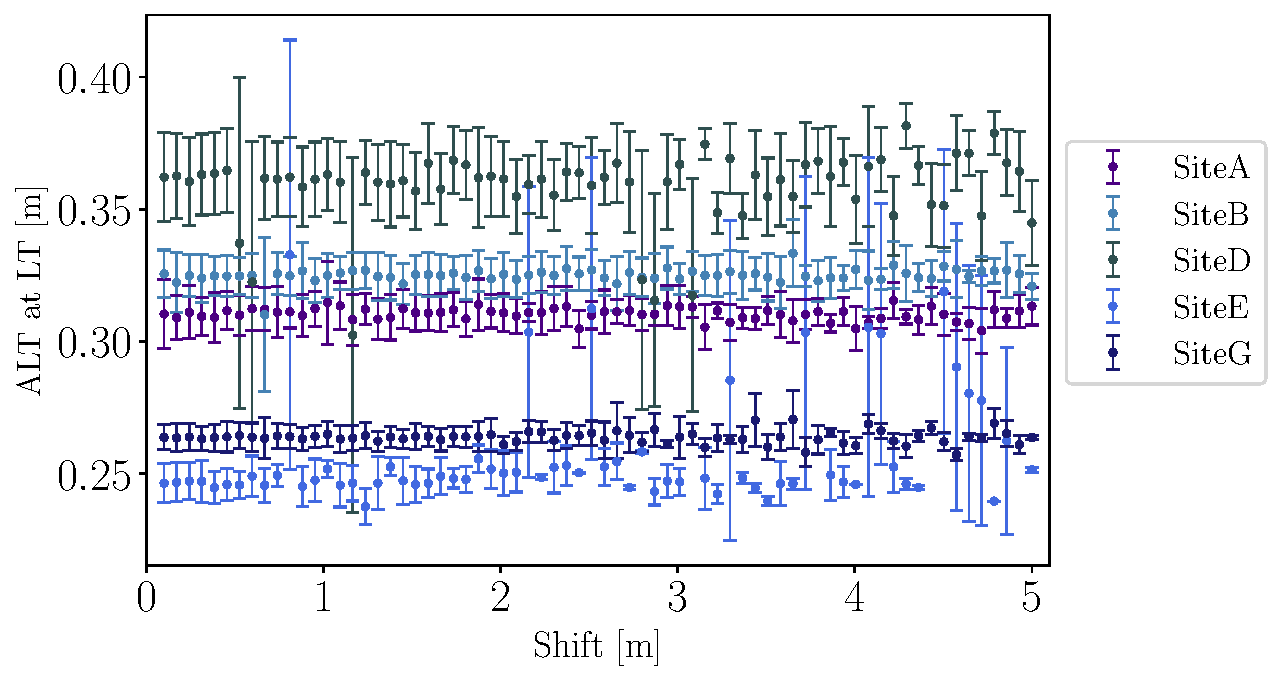
\includegraphics[width=0.85\textwidth]{AllCoresInOne_ALTvsShift.pdf}
	\caption[$\lambda_{\text{LT}}0$ vs. $s_{\text{sec}}$]{\small Annual layer thickness estimate at the depth section between Laki and Tambora, $\lambda_{\text{LT}}$ versus different shifts of the sections used in the spectral analysis.}
	\label{fig:AllCores_ALTvsShift}
\end{figure}




\section[Peak Detection]{Peak Detection}
\label{Sec:CompMeths_PeakDetection}

Knowing that water isotopic data are a proxy for temperature, the most obvious way to determine annual layers in the signals is by detecting peaks and troughs. During colder periods, e.g. winter, the air masses arriving at the ice core sites have formed more precipitation before reaching the sites, and the vapor that results in this final precipitation is then more depleted of heavy isotopes, resulting in lower isotopic values, troughs in Figure \ref{Fig:ICE_Crete_10m_dated}. The precipitation falling during warmer conditions, e.g. summer, is correspondingly less depleted of the heavy isotopes, and results in higher isotopic values, peaks in Figure \ref{Fig:COMPMETH_Crete_10m_PeaksTroughs}.
\begin{figure}[h]
	\centering
	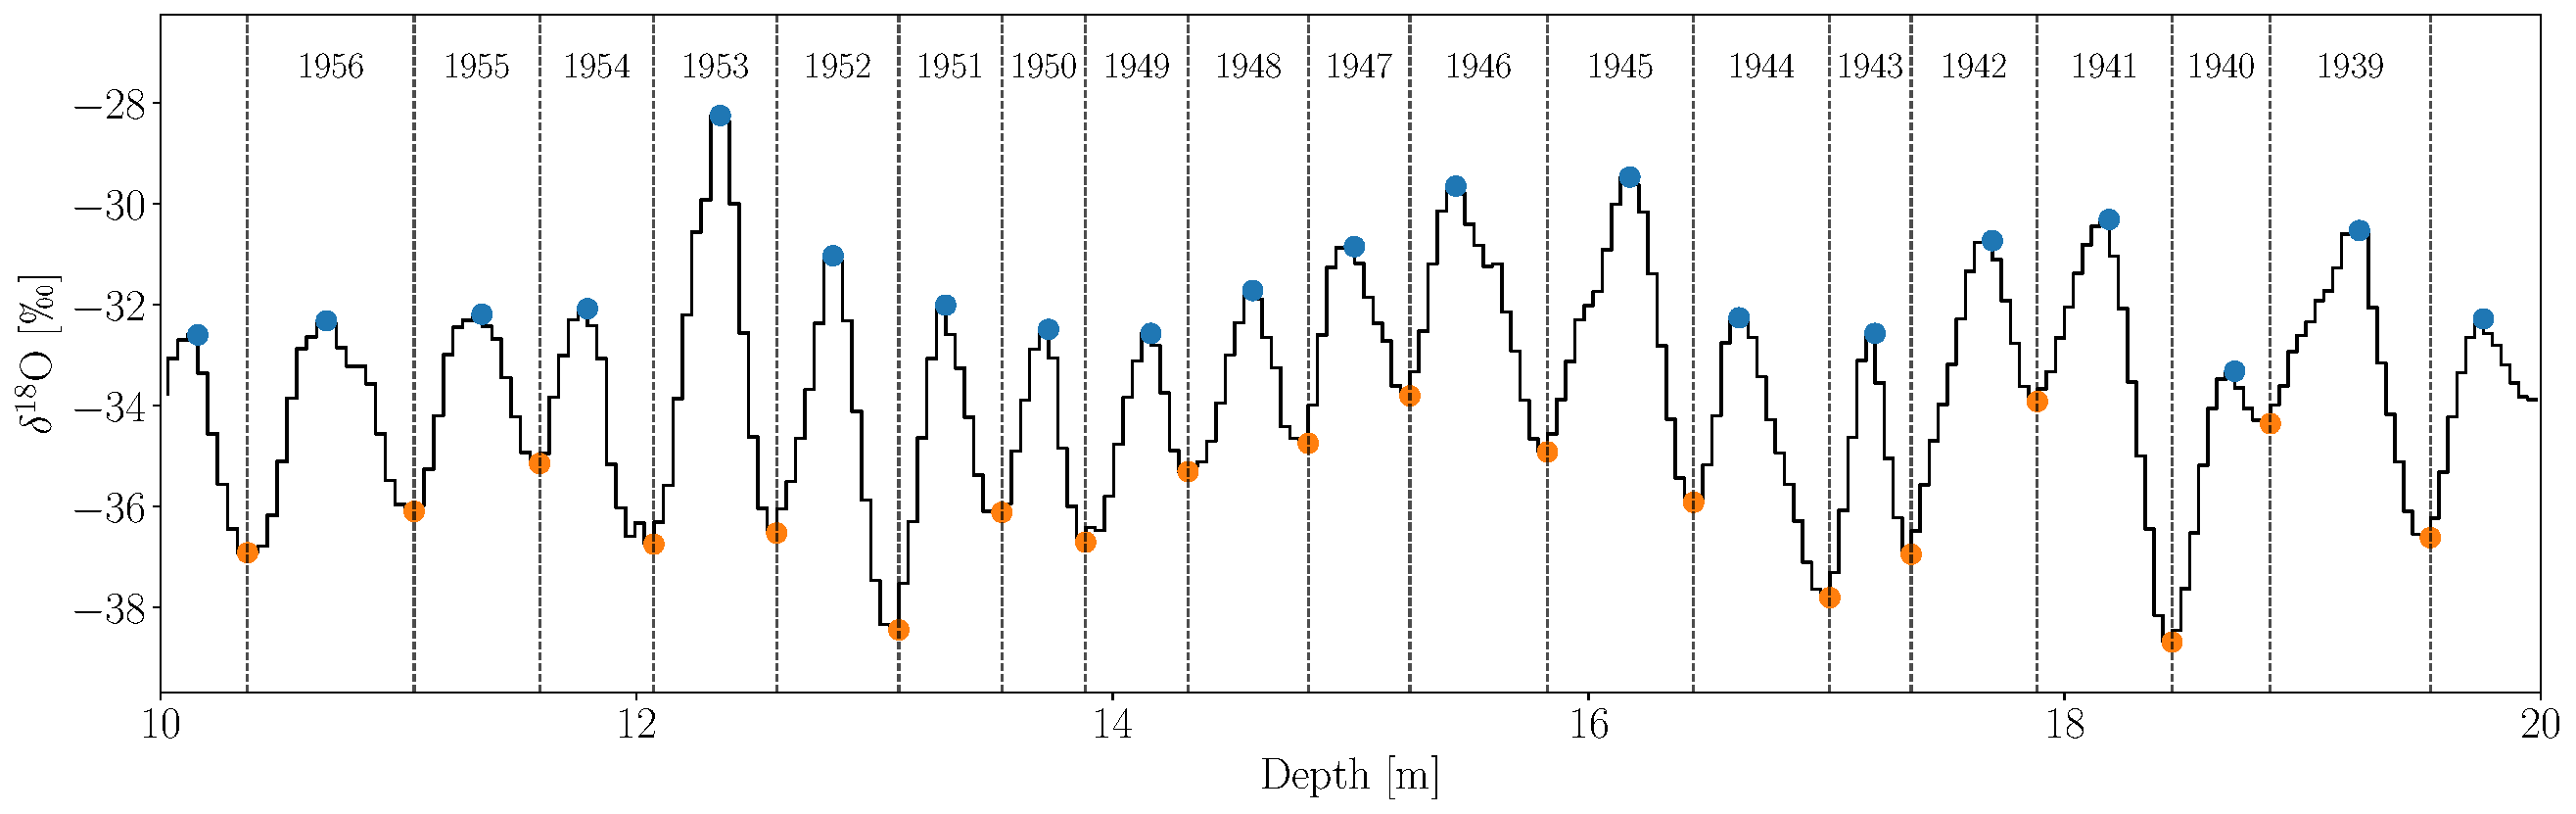
\includegraphics[width=\textwidth]{Crete_10m_PeaksTroughs.pdf}
	\caption[10 m of Crête core with peaks and troughs.]{\small Ten meters of the top of Cretê ice core, with identification and dating of 19 annual layers, with peaks(blue) corresponding to summers and troughs(orange) corresponding to winters.}
	\label{Fig:COMPMETH_Crete_10m_PeaksTroughs}
\end{figure}

Peak detection and layer counting has previously been carried out by visual inspection of the ice core depth signals, but as computers and algorithms have become more integrated in data analysis, it is now more common to use different computational methods. Developing and implementing layer counting and peak detection algorithms can be done in a number of different ways, but for this project, at first a very simple method has been initially implemented and later the method has been improved and optimized through a number of different constraints. One could also use different pattern recognition techniques[REFERENCE] to achieve more intelligent detection, and later some of these methods will be presented.

The most naïve approach, and the one first implemented in this project, to peak detection is to simply find local maxima by comparing neighbouring values. When examining point $d_i$, the point is deemed a local maxima, if $d_{i\pm1} < d_i$. Local minima, troughs, can be found in exactly the same manner by finding minima as $d_{i\pm1} > d_i$. A very simple constraint for this method is to keep a required minimal distance between peaks, so that two peaks cannot be detected within a point distance of $\Delta d_{\text{min}}$. For example at a depth of 12 m in Figure \ref{Fig:COMPMETH_Crete_10m_PeaksTroughs} two troughs can be seen, but only one is chosen, as they are within the threshold distance to each other, which here is set to $\Delta d_{\text{min}} = 7$ points. Here, the lowest of the two troughs is chosen. The threshold distance can be chosen in different ways, for this short section it has been chosen through visual inspection, but more generally it can be chosen by examining some of the intrinsic properties of the signal like the estimated $\lambda_A$, as explained in Section \ref{Subsubsec:SignalAnalysis_SpectralAnalysis_ALT}.



\section[Splines and Interpolation]{Splines and Interpolation}	
\label{Sec:CompMeths_SplinesAndInterpolation}
For the purpose of this thesis, interpolation of data needs to be fast, efficient and result in a function as smooth as possible. The last criterion is due to the knowledge of the nature of the data. The measurements are not continuous but should indeed in theory be so. Thus a good choice for interpolation of the data examined in this thesis would be the cubic spline interpolation. An instance of a such interpolation can be seen in Figure \ref{fig:Interp}.

\begin{figure}[h]
	\centering
	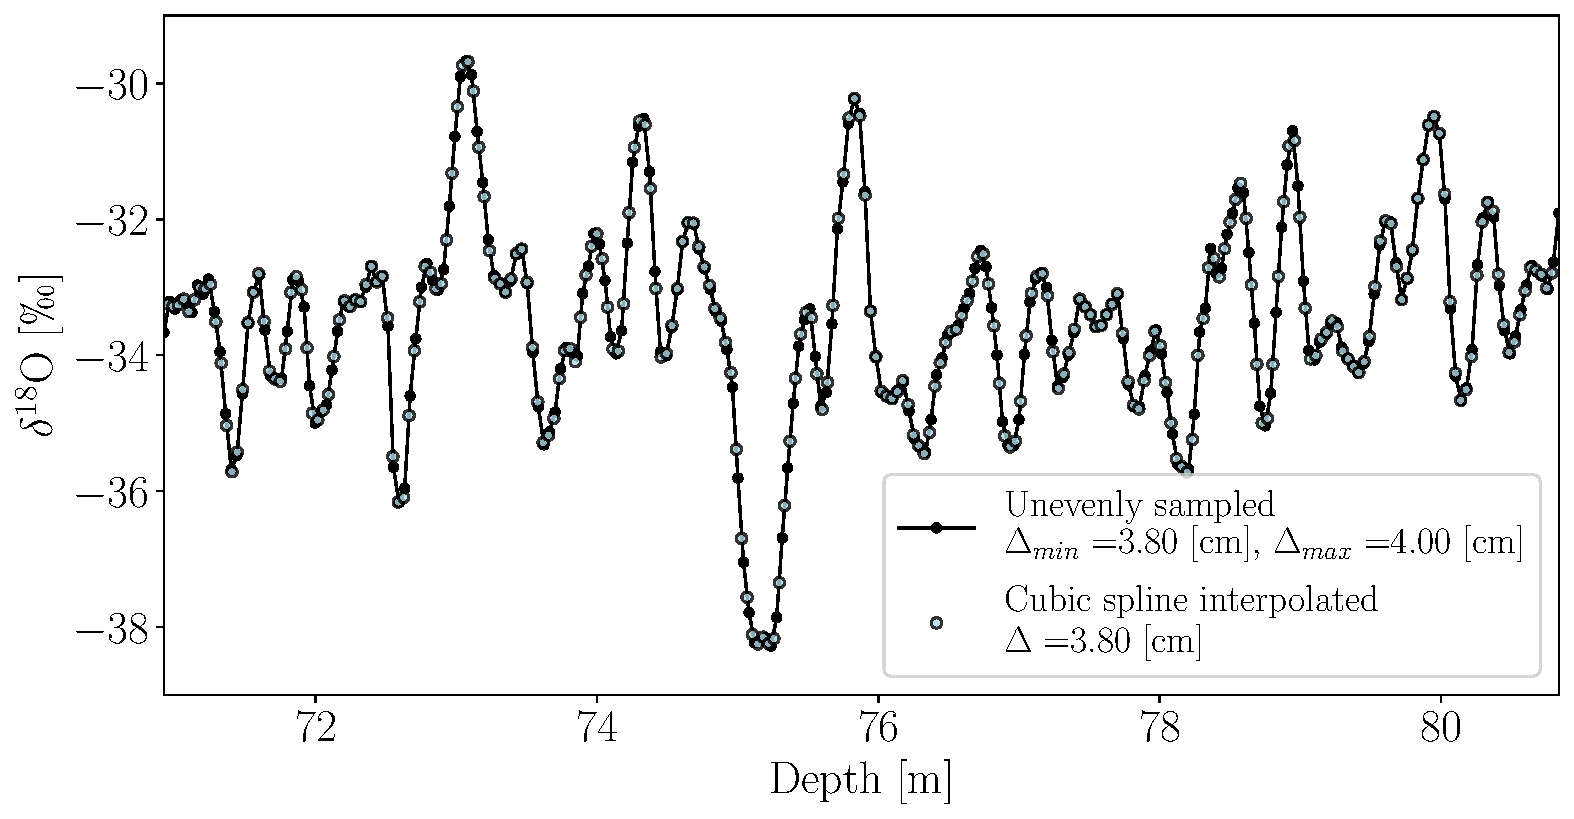
\includegraphics[width=\textwidth]{SiteA_DataSplineInterp.pdf}
	\caption[Even resampling of unevenly sampled data, Site A.]{\small Unevenly sampled signal from Site A resampled using cubic spline interpolation to an even signal with a new sample size equal to the minimum sample size found in the raw signal.}
	\label{Fig:COMPMETH_SiteA_DataSplineInterp}
\end{figure}

Cubic spline interpolation has been used in two instances during this analysis, both times through the \lstinline[language=Python]|Python SciPy| package \lstinline[language=Python]|scipy.interpolate.CubicSpline|. Firstly, to assure equally spaced data points, so as to be able to perform a useful frequency analysis through spectral transformation, see Section, \ref{sec:???}. Secondly cubic spline interpolation was used to improve on peak detection in the final back diffused data. The final data have a rather low resolution, leading to an initial guess of peak positioning that might be shifted due to the discretization. Through cubic spline interpolation it is possible to construct a smooth estimate of a signal of higher resolution, leading to a peak positioning estimate that might be less shifted, see Figure \ref{fig:InterpFinal}.


\subsection[Interpolation][Interpolation]{Interpolation}
\label{Subsec:CompMeths_SplinesAndInterpolation_Interpolation}
\begin{figure}[h]
	\centering
	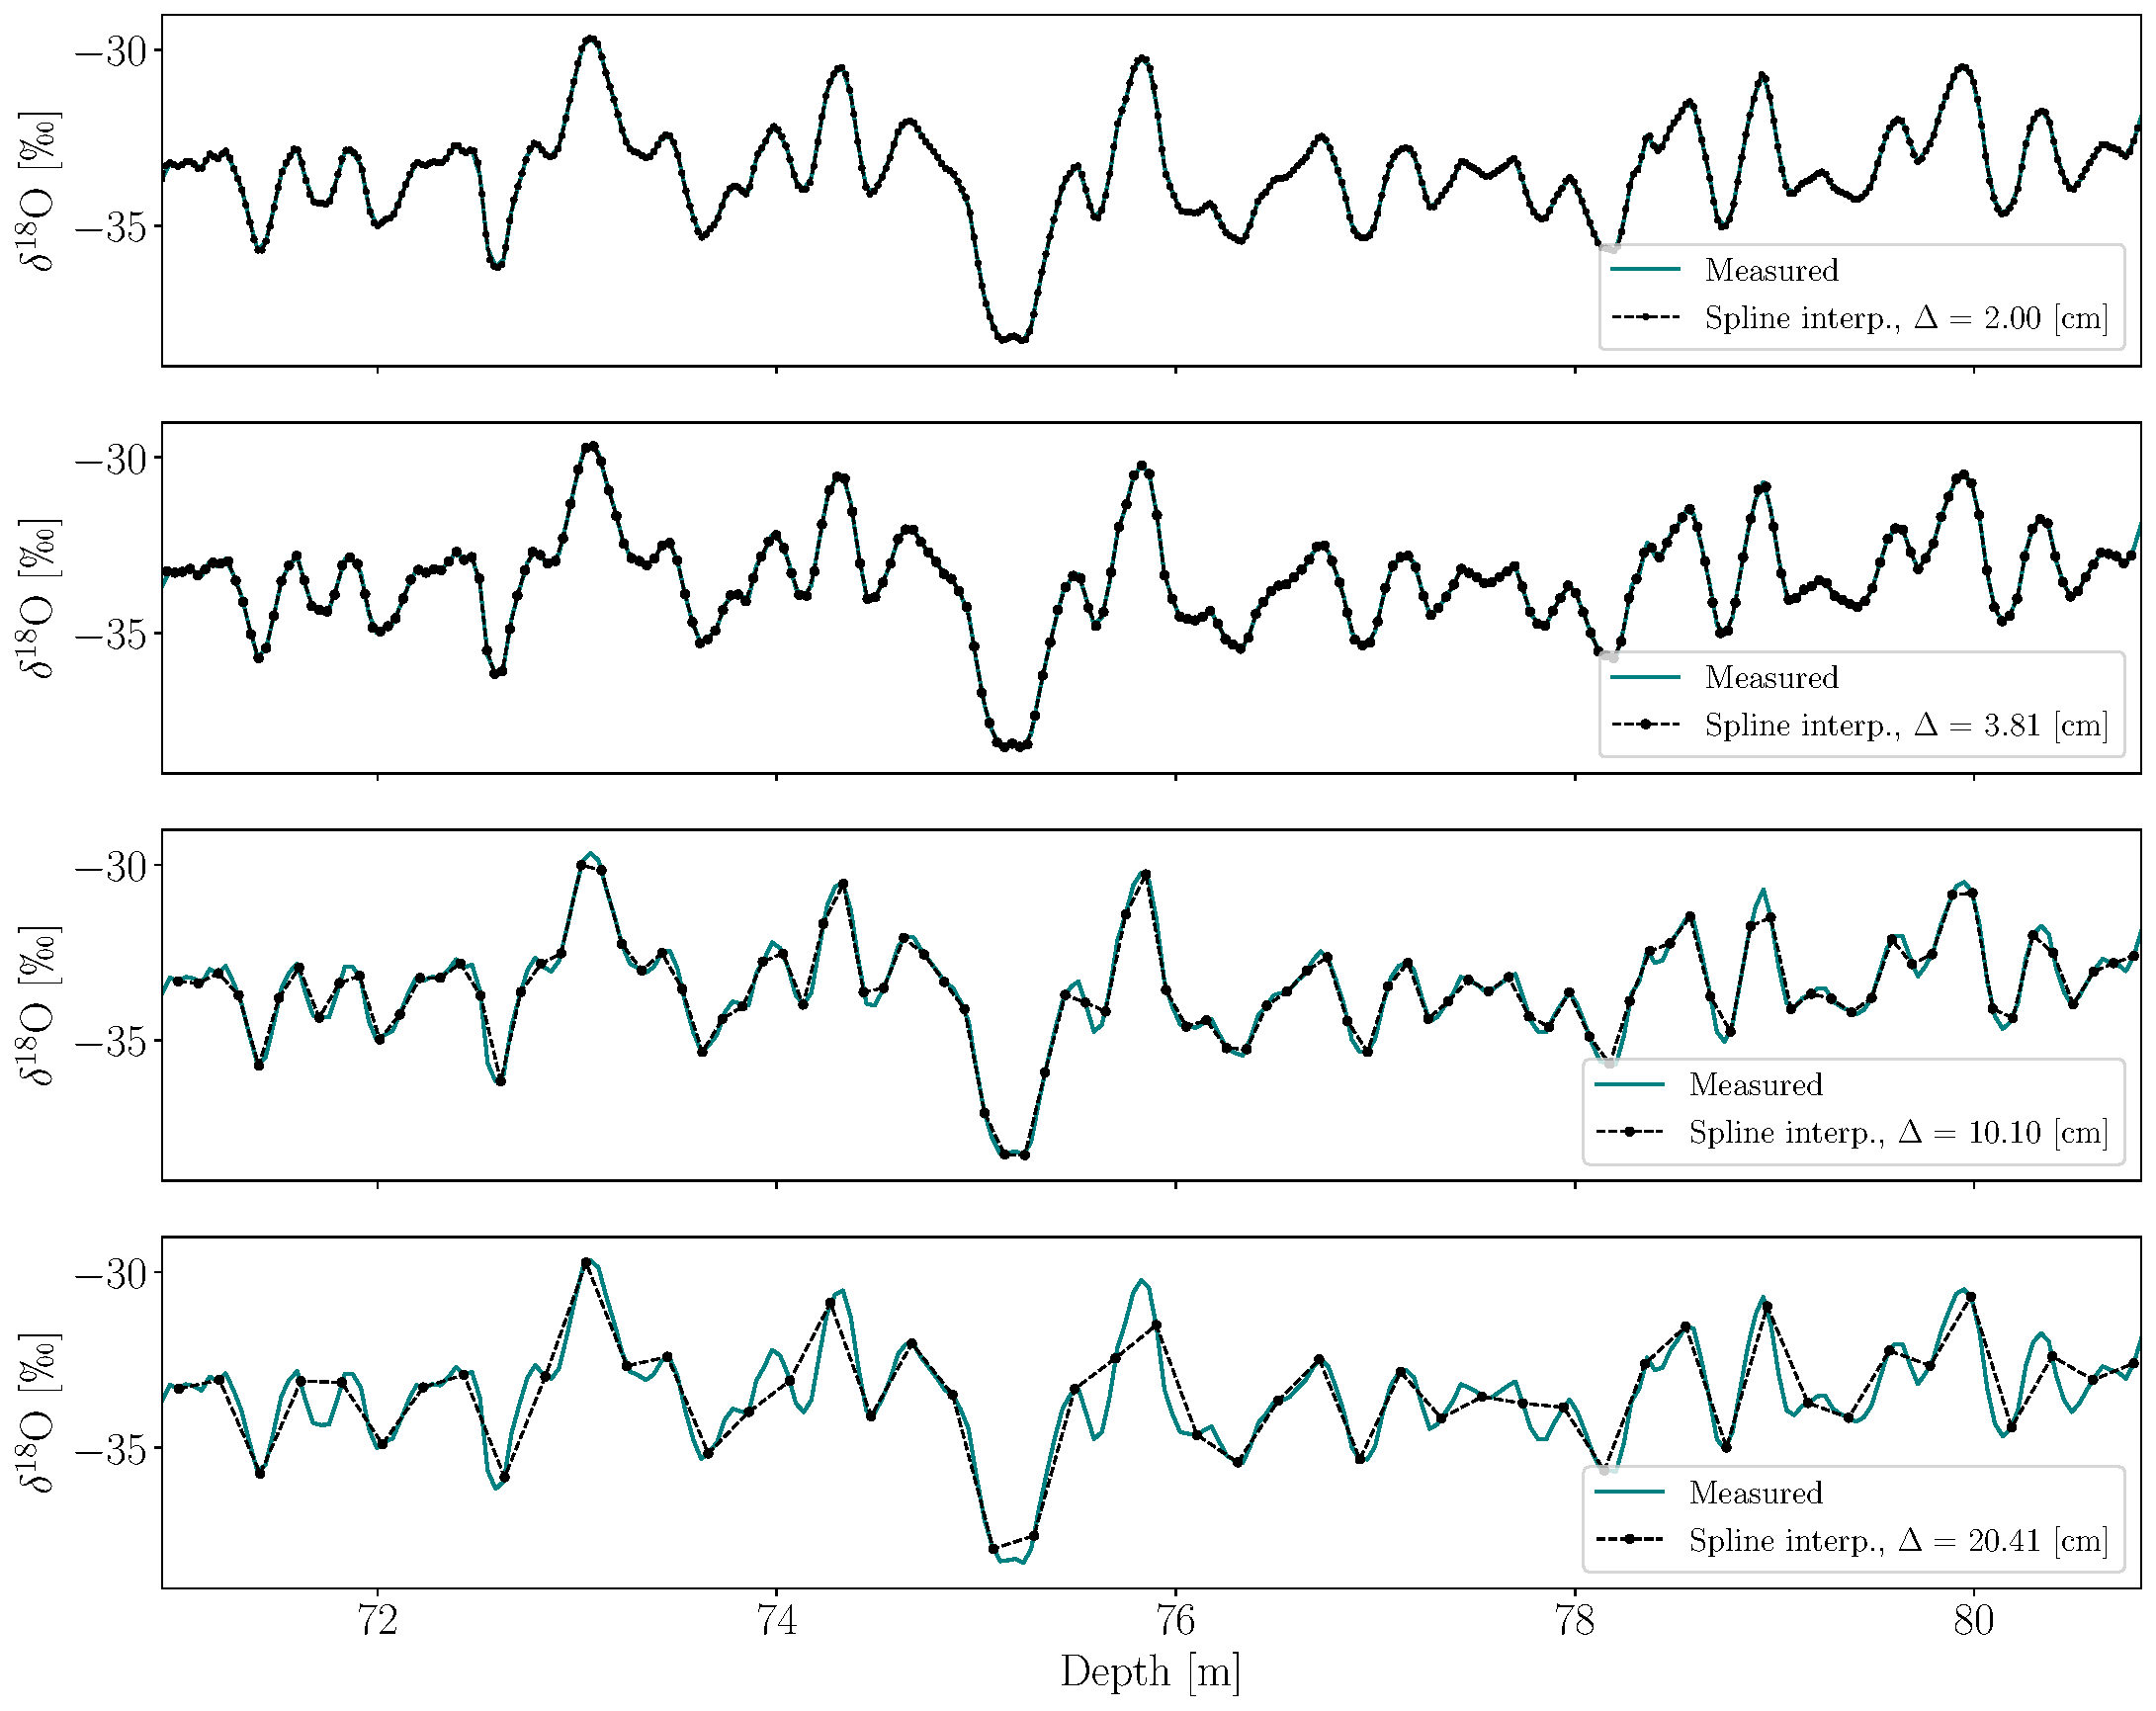
\includegraphics[width=\textwidth]{SiteA_MultiSplineInterp.pdf}
	\caption[Different resamplings of Site A.]{\small Four different resampled signals of Site A data, showing loss of information when resampling resolution is low.}
	\label{Fig:COMPMETH_SiteA_MultiSplineInterp}
\end{figure}
Interpolation is a tool that can be used - and misused - to extract more information out of a given set of data. Used correctly, interpolation can reveal more information than is initially available and disclose connections not apparent at first, but used incorrectly, it can be manipulated to infer misleading correlations and lead to inaccurate conclusions. Thus it is a tool that must be used with care. Aiming to avoid incorrect deductions and inferences one should at first gain as much knowledge about the data at hand as possible. By understanding how the data have come about and gaining knowledge about the underlying physical theories a somewhat deficient data set can robustly and securely be interpolated to accommodate the needs of the analysis. In the case of this thesis, both knowledge about data gathering and the physics at play have been gained and thus some of the common fallacies may be avoided. The limits of the data available is due to the discrete sampling, leading to a minimum sampling of about 26 samples per meter of ice.

When considering that the depth series of 33 years between Tambora and Laki is just above 10 meters, this means that each meter of ice needs to contain at least three years on average. 26 samples per three years might not sound as a bad sampling interval, but if the goal is to show seasonality and give a best estimate of annual layer thickness, interpolation could be put to good use to be able to give better estimates of the exact placement of peaks and troughs.




%\subsubsection[Basic Idea][Basic Idea]{Basic Idea}
%\label{Subsubsec:CompMeths_SplinesAndInterpolation_Interpolation_BasicIdea}
%\todo{Write short introduction to interpolation here. Reference Appendix.}

\subsection[Interpolation in this Project][Interpolation in this Project]{Cubic Spline Interpolation in this Project}
\label{Subsec:CompMeths_SplinesAndInterpolation_InterpolationInThisProj}
An in depth description of interpolation and splines can be found in Appendix \ref{Appendix V: Splines and Interpolations}. In general, these interpolation methods are implemented and examined in two particular sections of the analysis: 
\begin{enumerate}
	\item Cubic spline interpolation of raw, uneven data to represent even data, that can be analyzed through fast spectral transforms.
	\item Cubic spline interpolation of the final back-diffused signal estimate to enhance resolution for more efficient peak detection.
\end{enumerate}

The effects of both interpolation methods are presented in the following chapter, in Section \ref{Subsec:METH_Interpolation}







\end{document}
